\documentclass{article}
\usepackage{setspace}
\usepackage{natbib}
% Language setting
\usepackage{subfig}
\usepackage[english]{babel}
\usepackage{float}

% Set page size and margins
% Replace `letterpaper' with `a4paper' for UK/EU standard size
\usepackage[letterpaper,top=2cm,bottom=2cm,left=3cm,right=3cm,marginparwidth=1.75cm]{geometry}

% Useful packages
\usepackage{amsmath}
\usepackage{graphicx}
\usepackage[colorlinks=true, allcolors=blue]{hyperref}


\begin{document}


\section{Supplemental Figures}
\subsection{SUMO1}
% QC results for SUMO1
% logphi bias plot
\begin{figure}[H]%
    \centering
    \subfloat[\centering the $log(\phi)$ bias plot]{{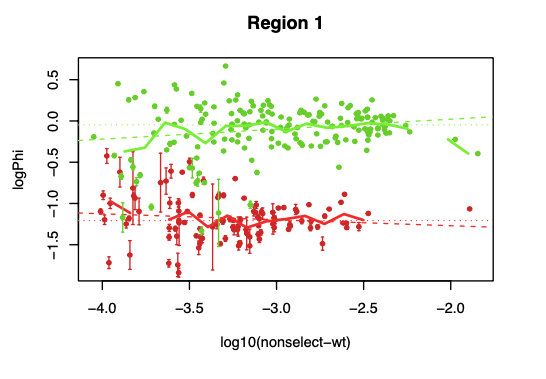
\includegraphics[width=.45\textwidth]{Figures/SUMO1/logphi_bias.png} }}%
    \qquad
    \subfloat[\centering filtering breakdown]{{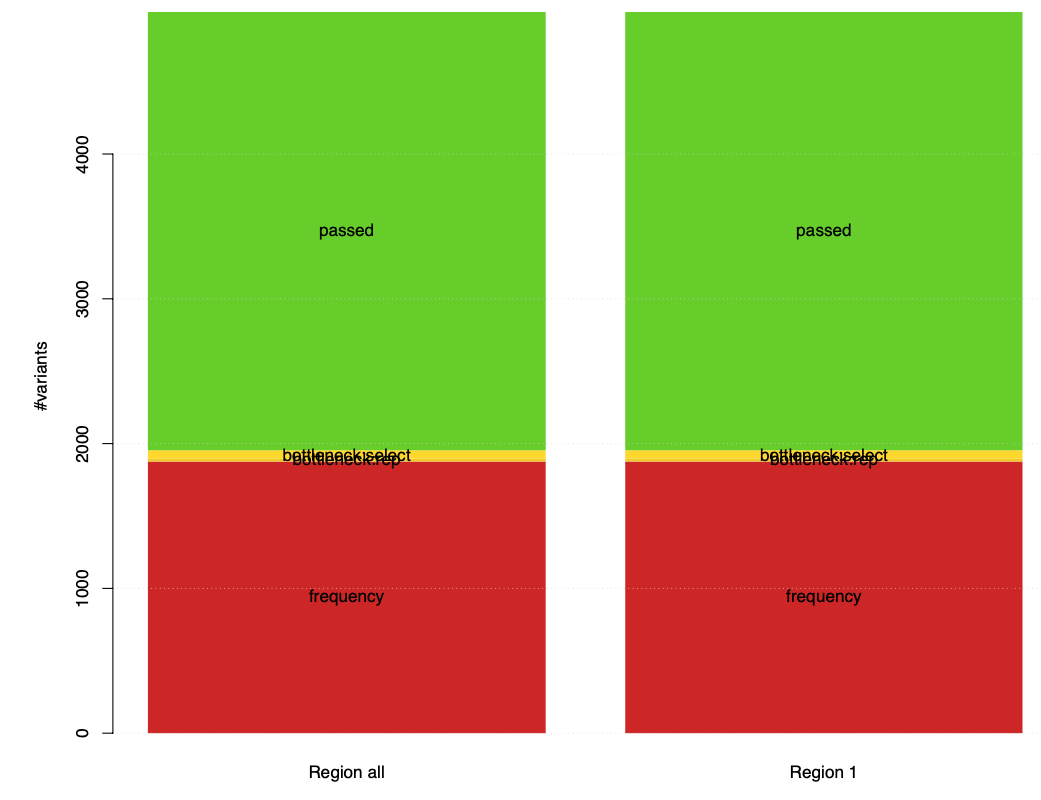
\includegraphics[width=.45\textwidth]{Figures/SUMO1/filtering.png} }}%
    \caption{The $log(\phi)$ bias plot and the filtering breakdown bar plot for SUMO1 map. The $log(\phi)$ bias plot illustrates how the $\log(\phi)$ values of synonymous(green) and nonsense(red) variants changing as the read frequency cutoff increasing. The filtering breakdown plot show the number of SUMO1 variants in region 1 that were subjected to individual filters, including the frequency filter (excludes variants that have low marginal frequencies); the bottleneck:rep filter excludes variants have low correlation with their replicates; and the bottleneck:select filter excludes variants that have frequency drop-out in the selection condition.}%
    \label{fig:filtering}%
\end{figure}



% coverage heatmap 
\begin{figure}[H]%
    \centering
    \subfloat[\centering coverage heatmap]{{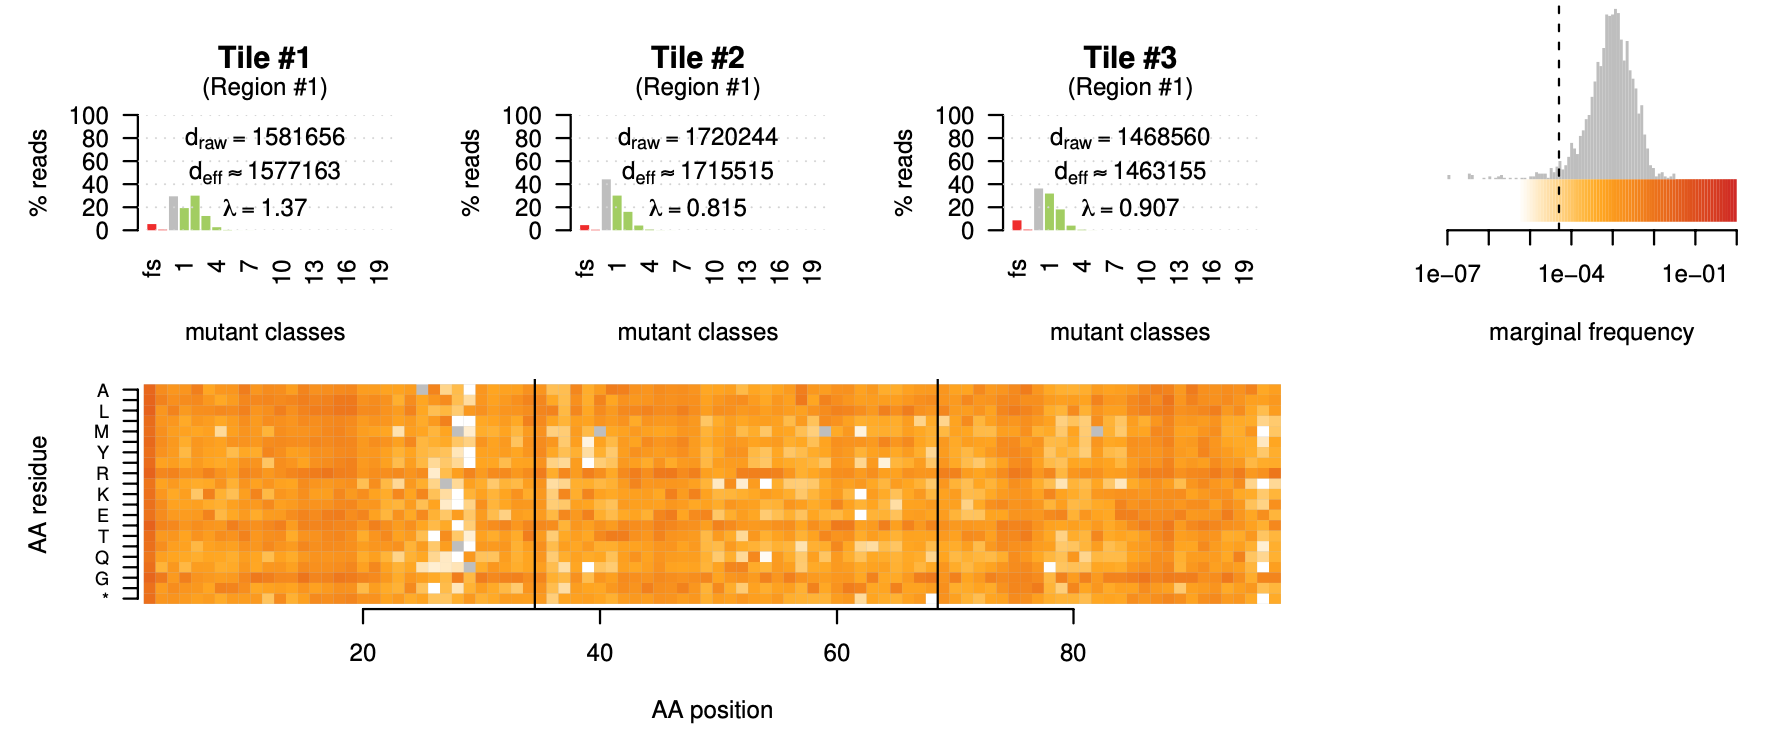
\includegraphics[width=.6\textwidth]{Figures/SUMO1/SUMO_coverage.png} }}%
    \qquad
    \subfloat[\centering Extrapolation for region 1]{{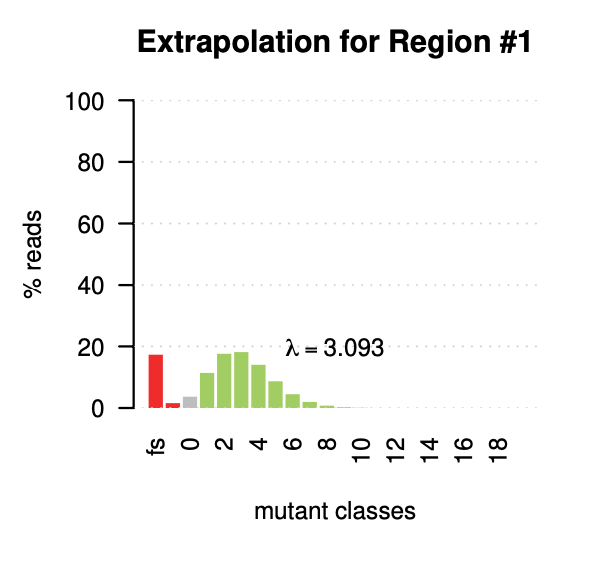
\includegraphics[width=.3\textwidth]{Figures/SUMO1/Extrapolation_R1.png} }}%
    \caption{The coverage heatmap and an extrapolation of the number of variants per clone for Region 1 for the re-calculated SUMO1 map. The heatmap shows marginal frequencies for each amino acid change. $\lambda$ refers to the mean of the best fitting Poisson distribution of the number of variants observed per read.}%
    \label{fig:heatmap}%
\end{figure}

% the standard error for SUMO1
\begin{figure}[H]
    \centering
    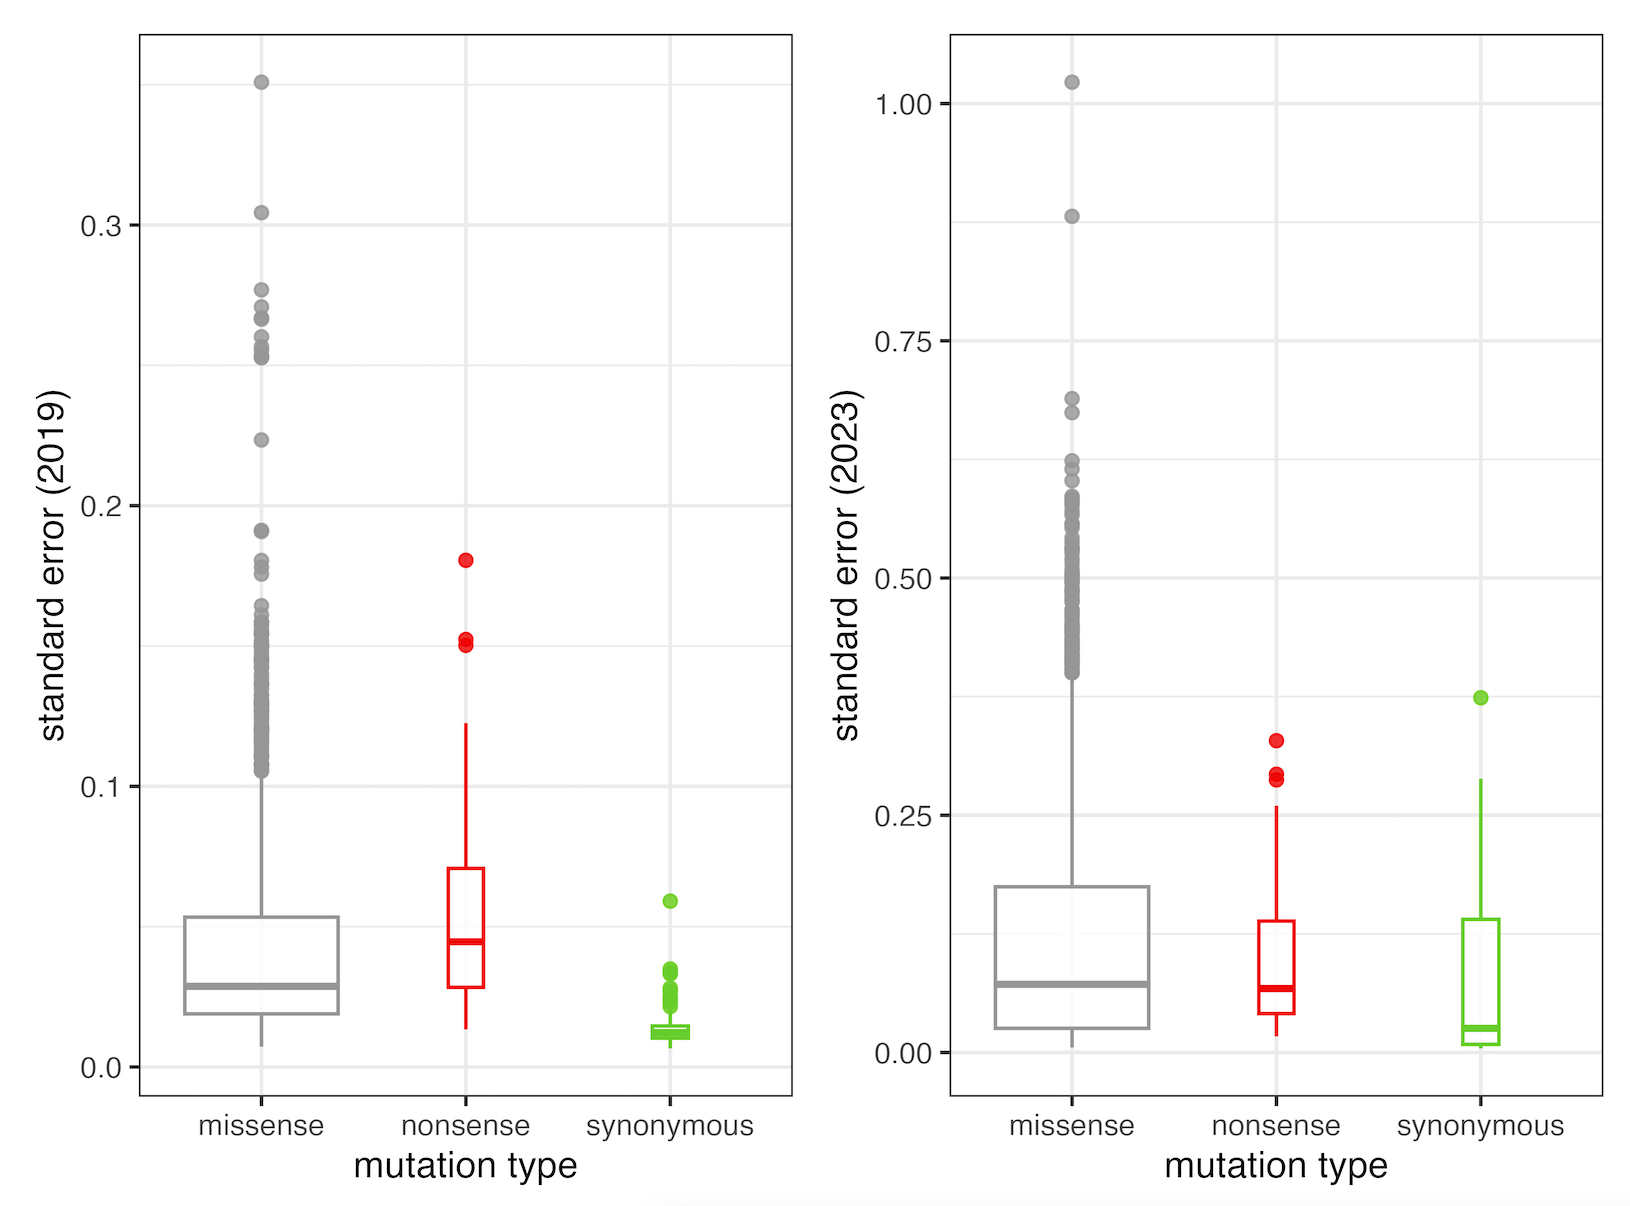
\includegraphics[width =.8\textwidth]{Figures/SUMO1/standard_error.png}
    \caption{The distribution of standard error of fitness scores produced by the Legacy (2019) Tileseq pipelines and the TileseqPro (2023) pipelines.}
    \label{fig:se boxplot}
\end{figure}

% fitness score comparison
\begin{figure}[H]%
    \centering
    \subfloat[\centering ]{{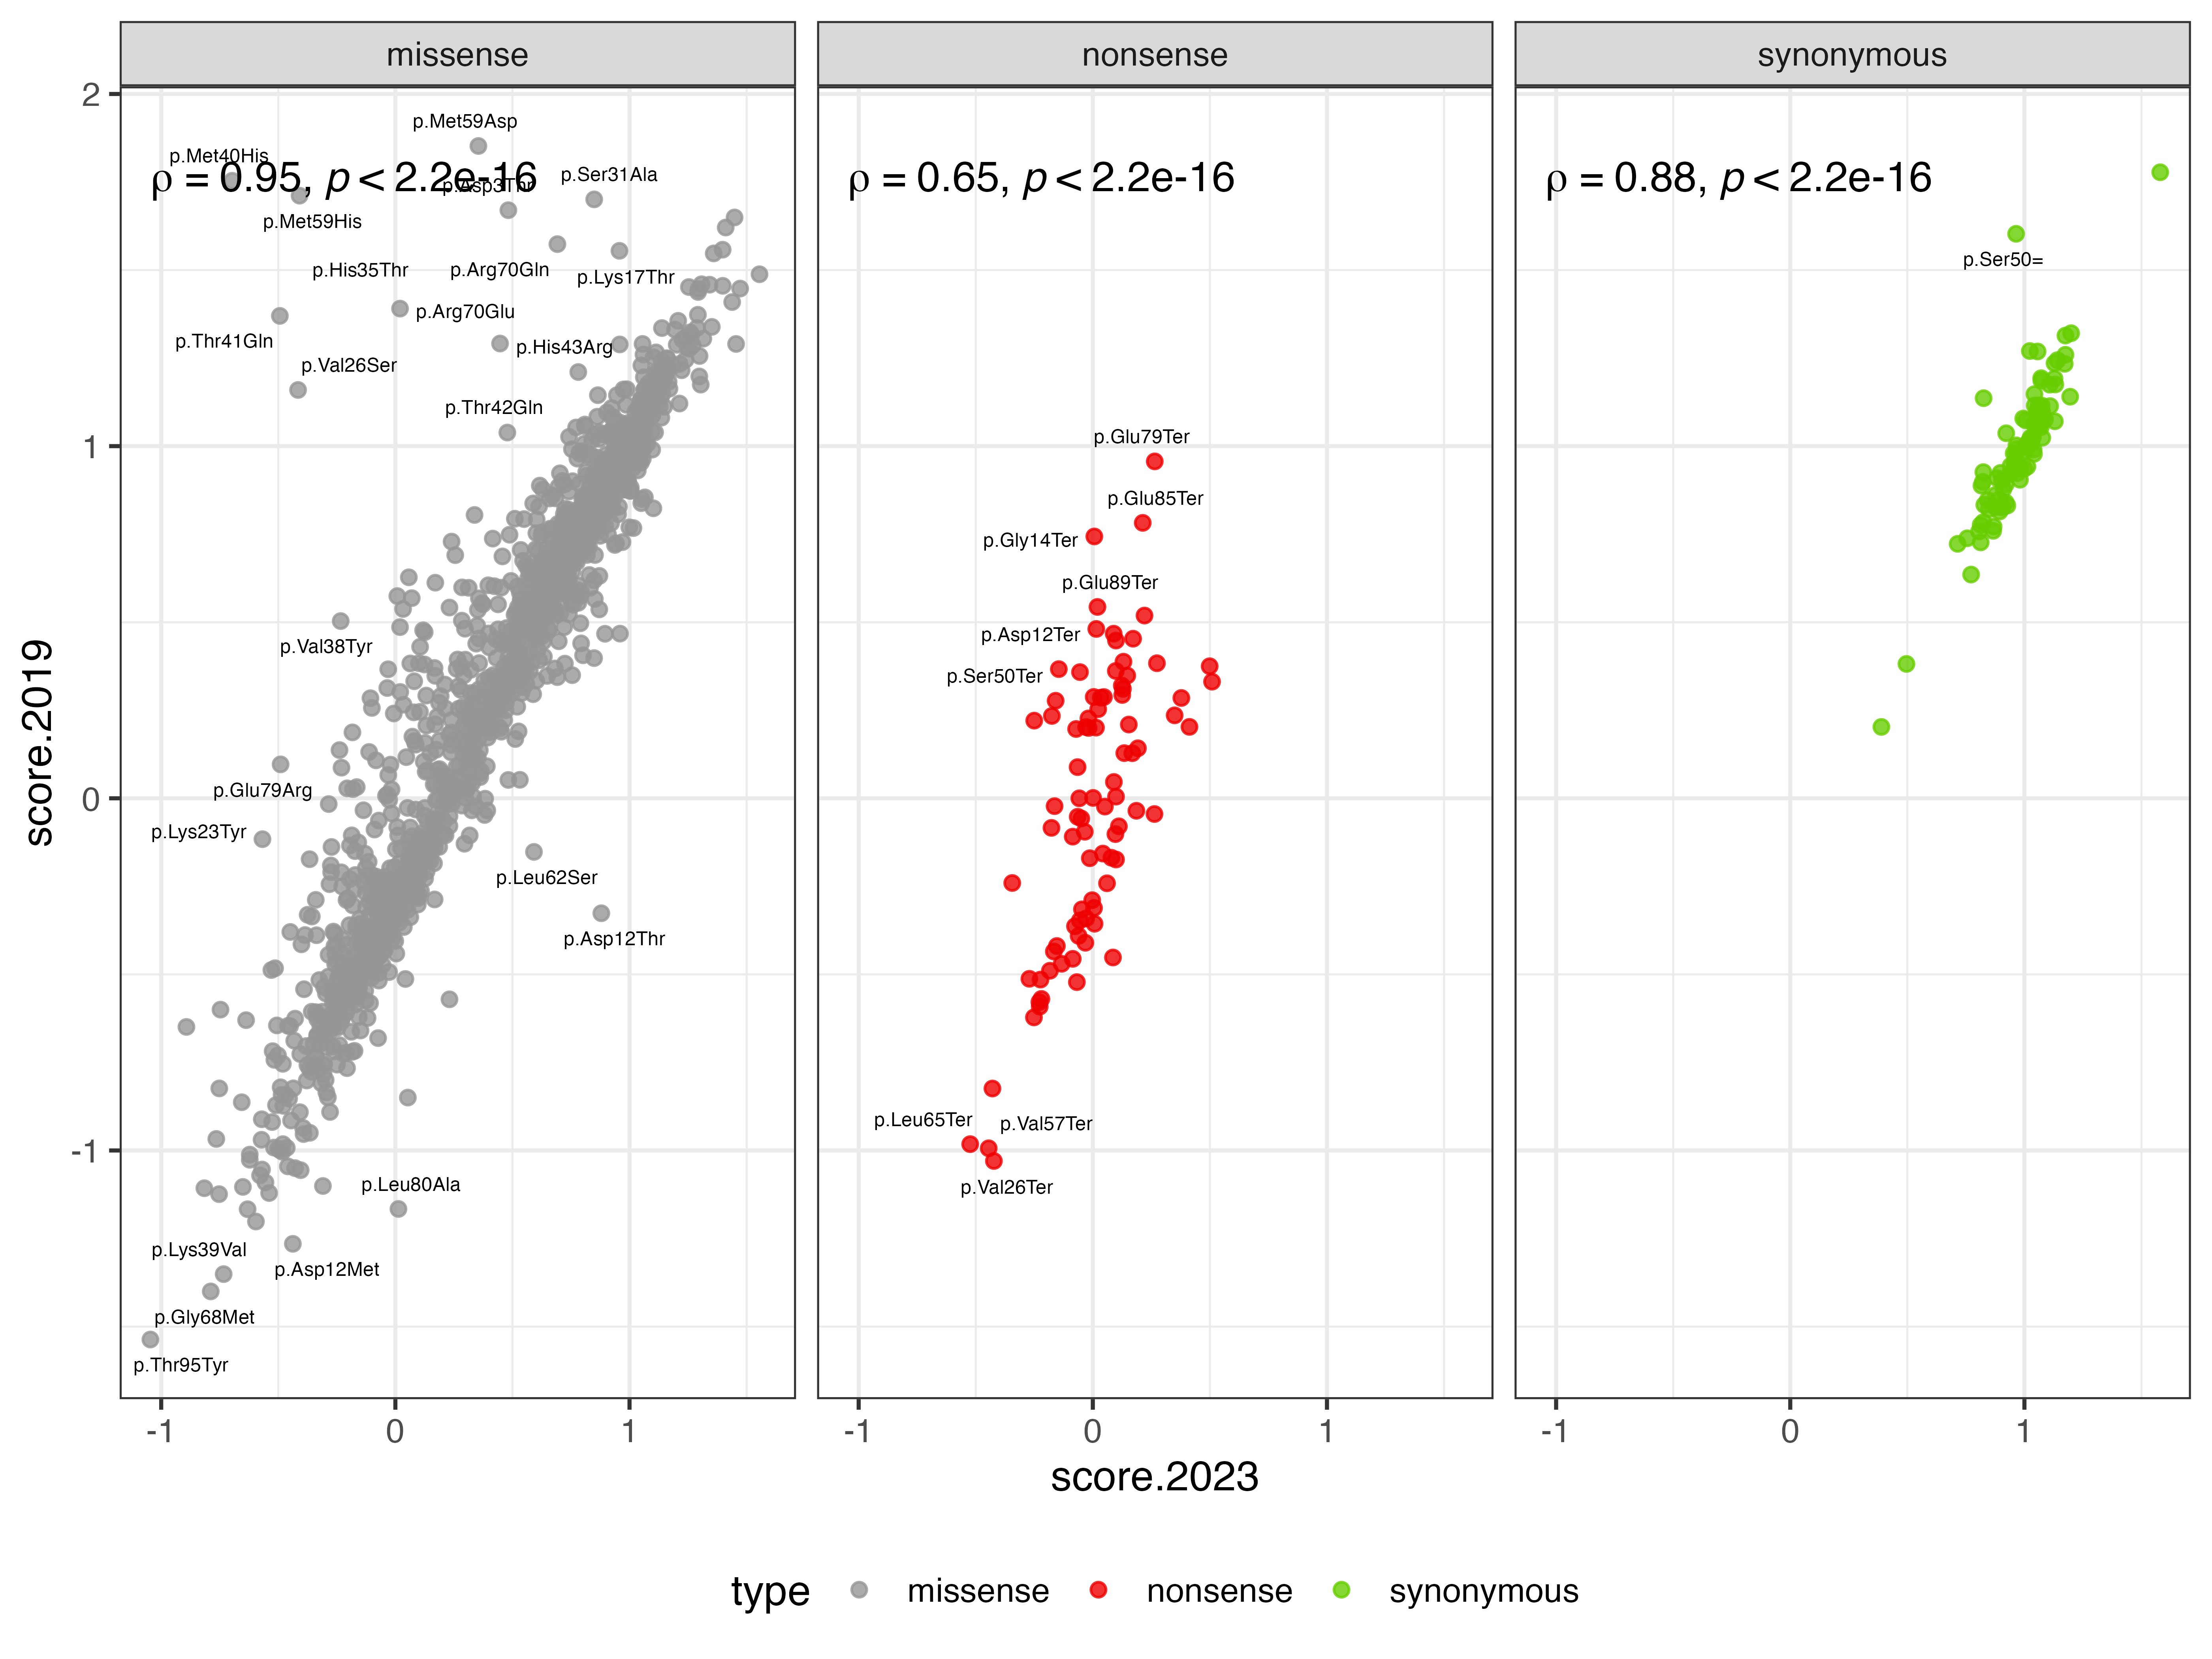
\includegraphics[width=.57\textwidth]{Figures/SUMO1/comparison_mutation.png} }}%
    \qquad
    \subfloat[\centering ]{{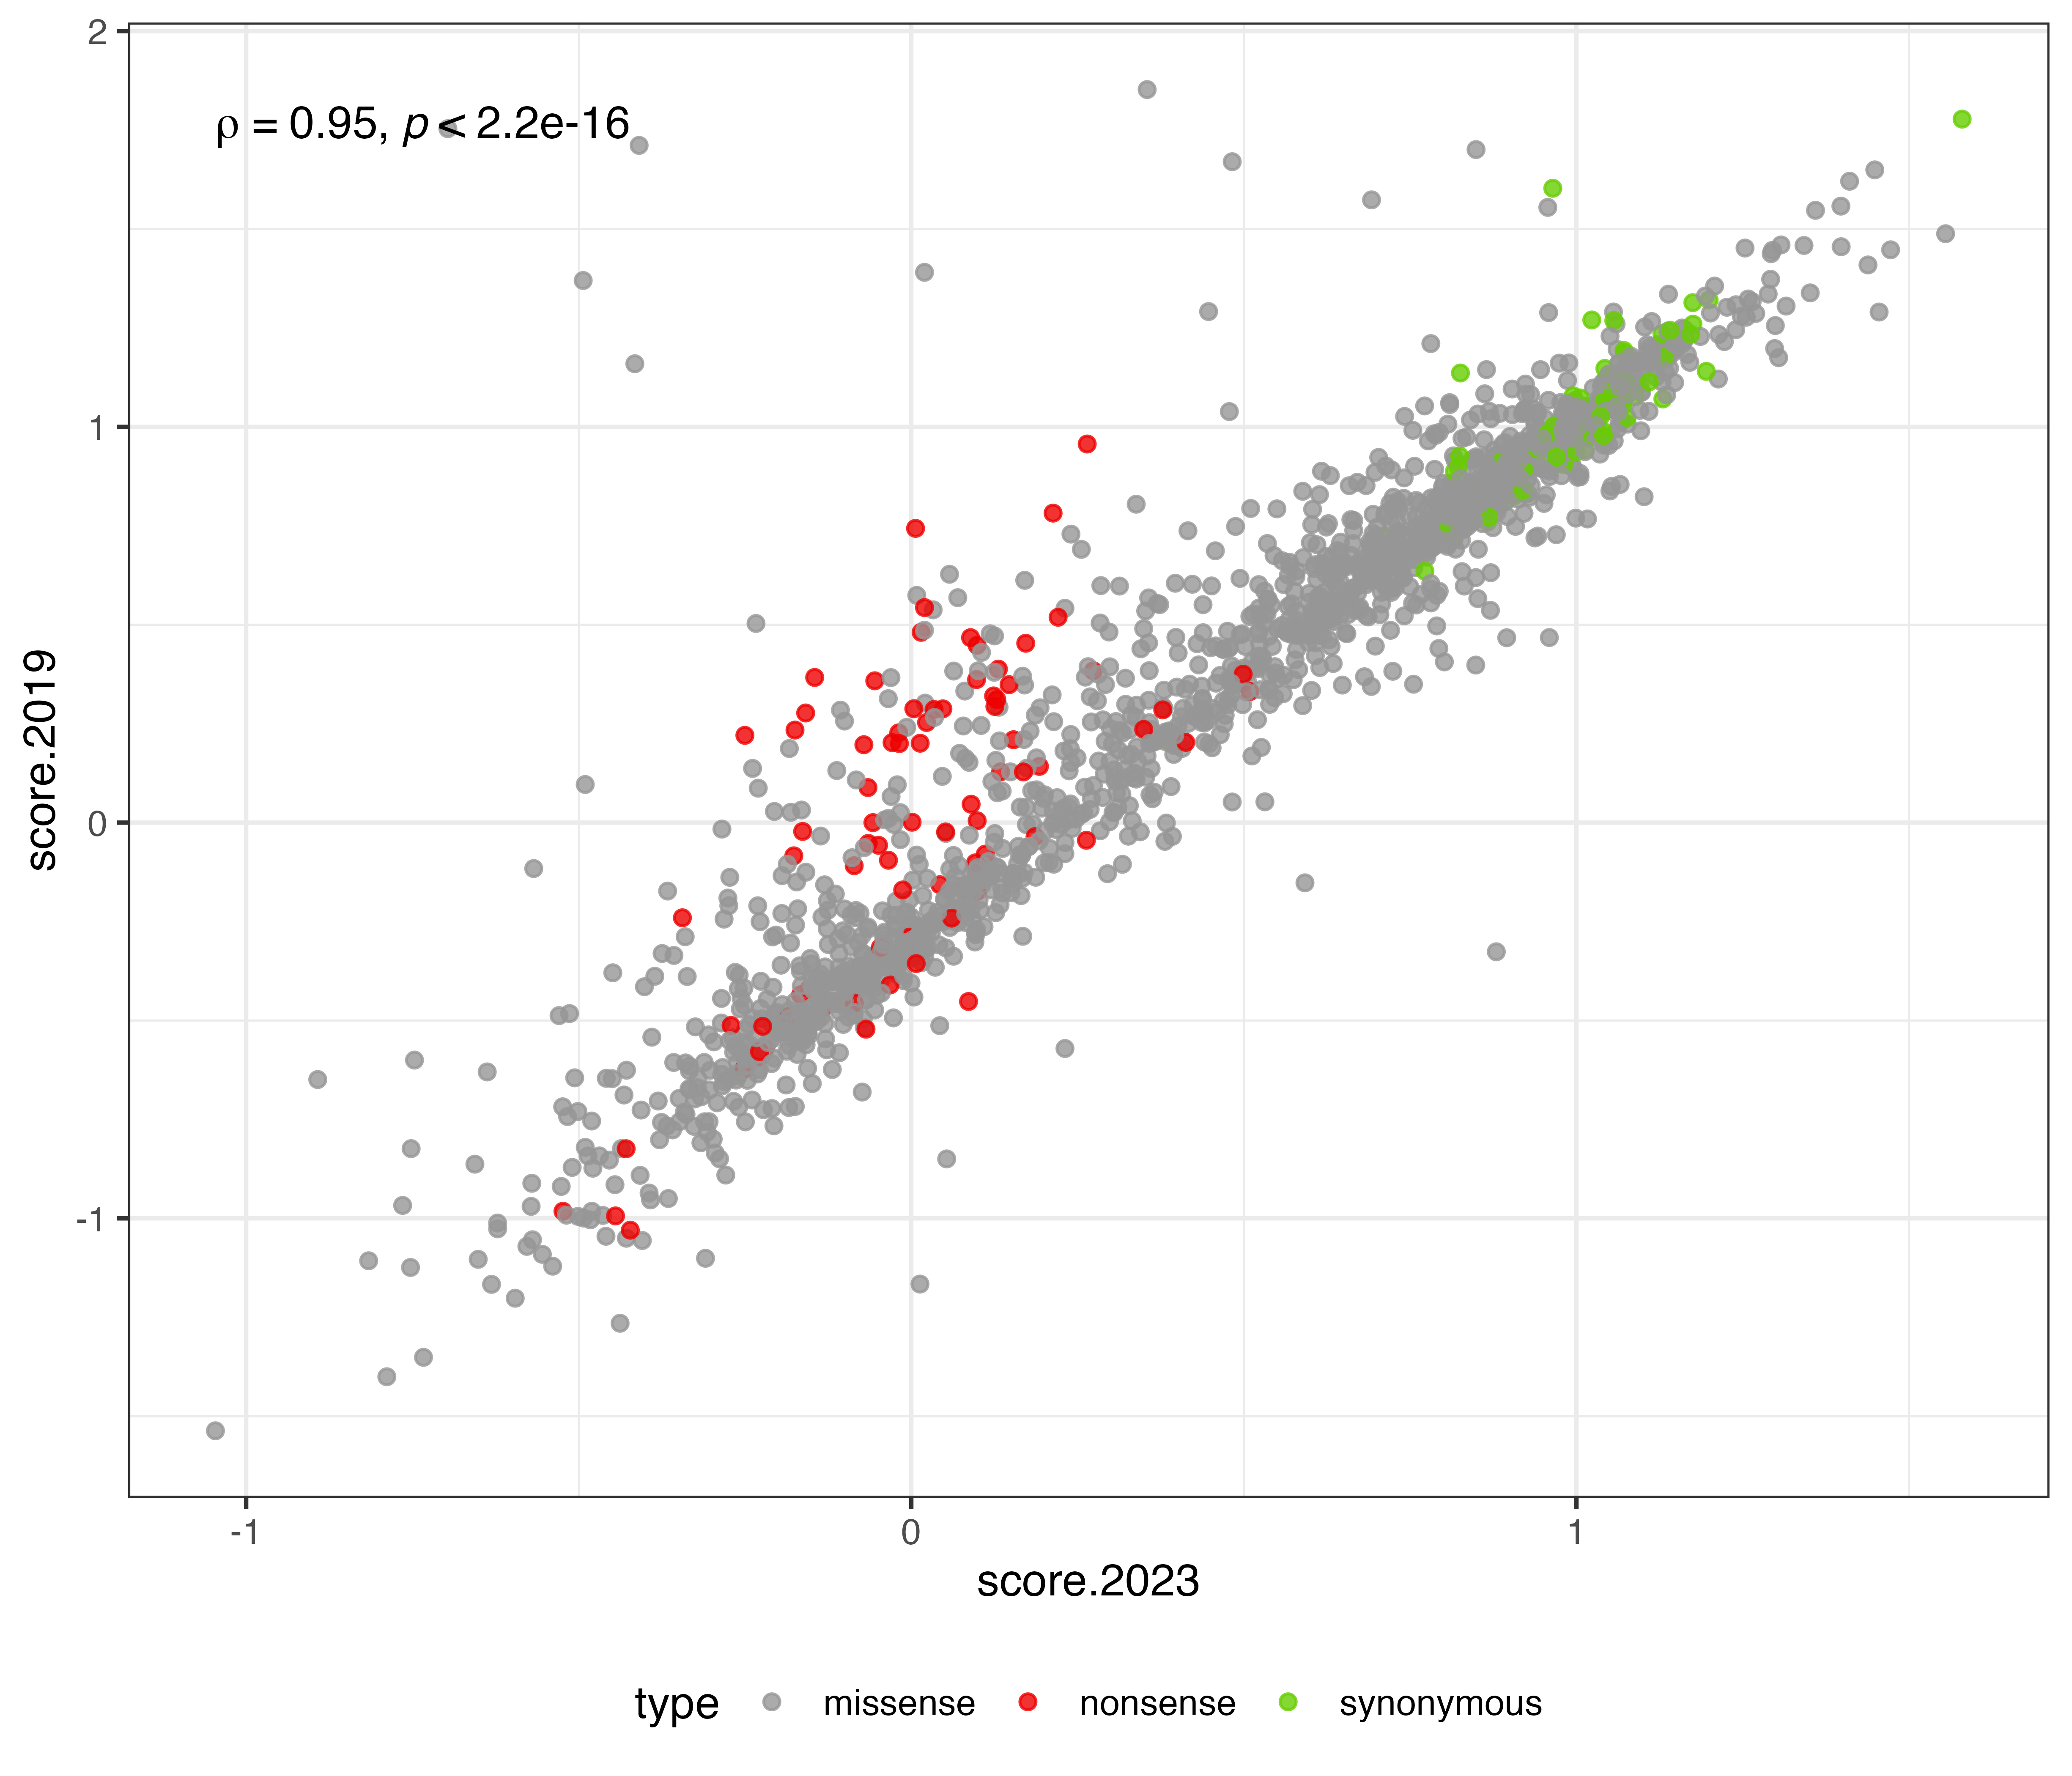
\includegraphics[width=.57\textwidth]{Figures/SUMO1/comparison_overall.png} }}%
    \qquad
    \subfloat[\centering ]{{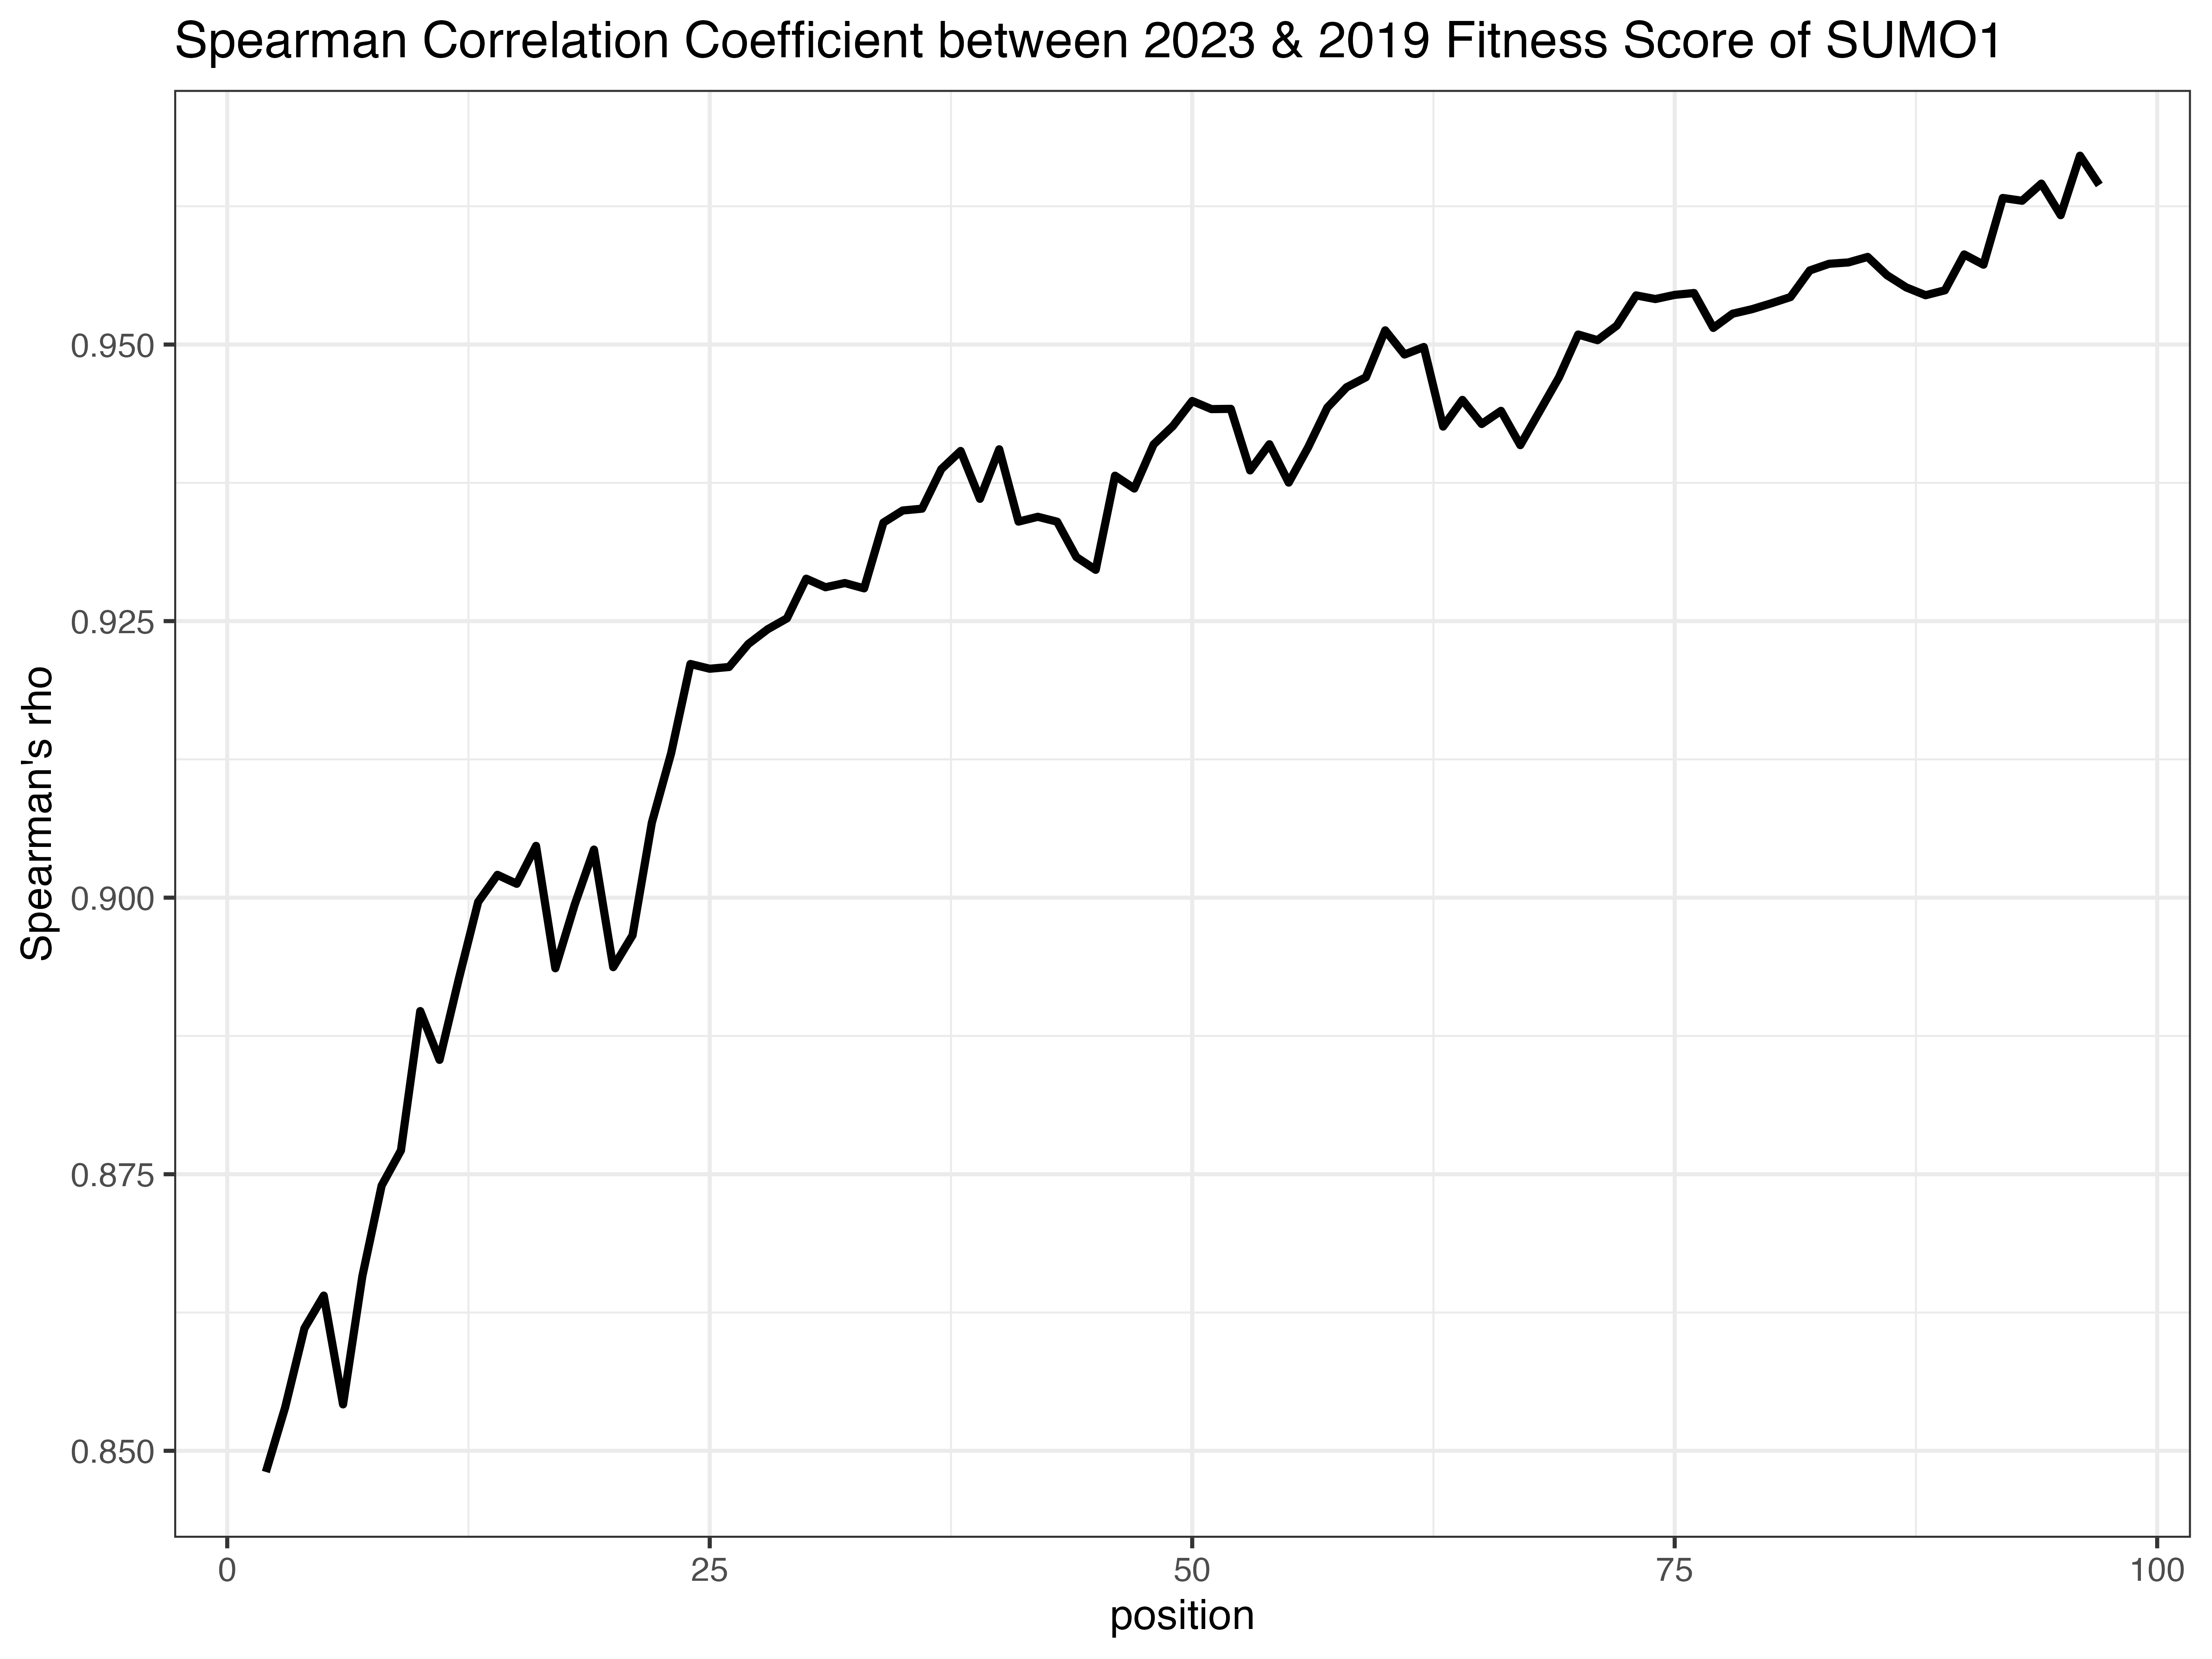
\includegraphics[width=.57\textwidth]{Figures/SUMO1/spearman_score.png} }}%
    \caption{Correlation between TileseqPro and Legacy scores. (a) and (b) show scatter plots for the two versions of fitness scores of SUMO1 with missense variants in gray, nonsense variants in red and synonymous variants in green, (c) Moving window analysis of Spearman's $\rho$ between new and old scores along amino acid position.}%
    \label{fig:scatter plot}%
\end{figure}

\subsection{CALM1}
% CALM1 coverage

\begin{figure}[H]%
    \centering
    \subfloat[\centering coverage heatmap]{{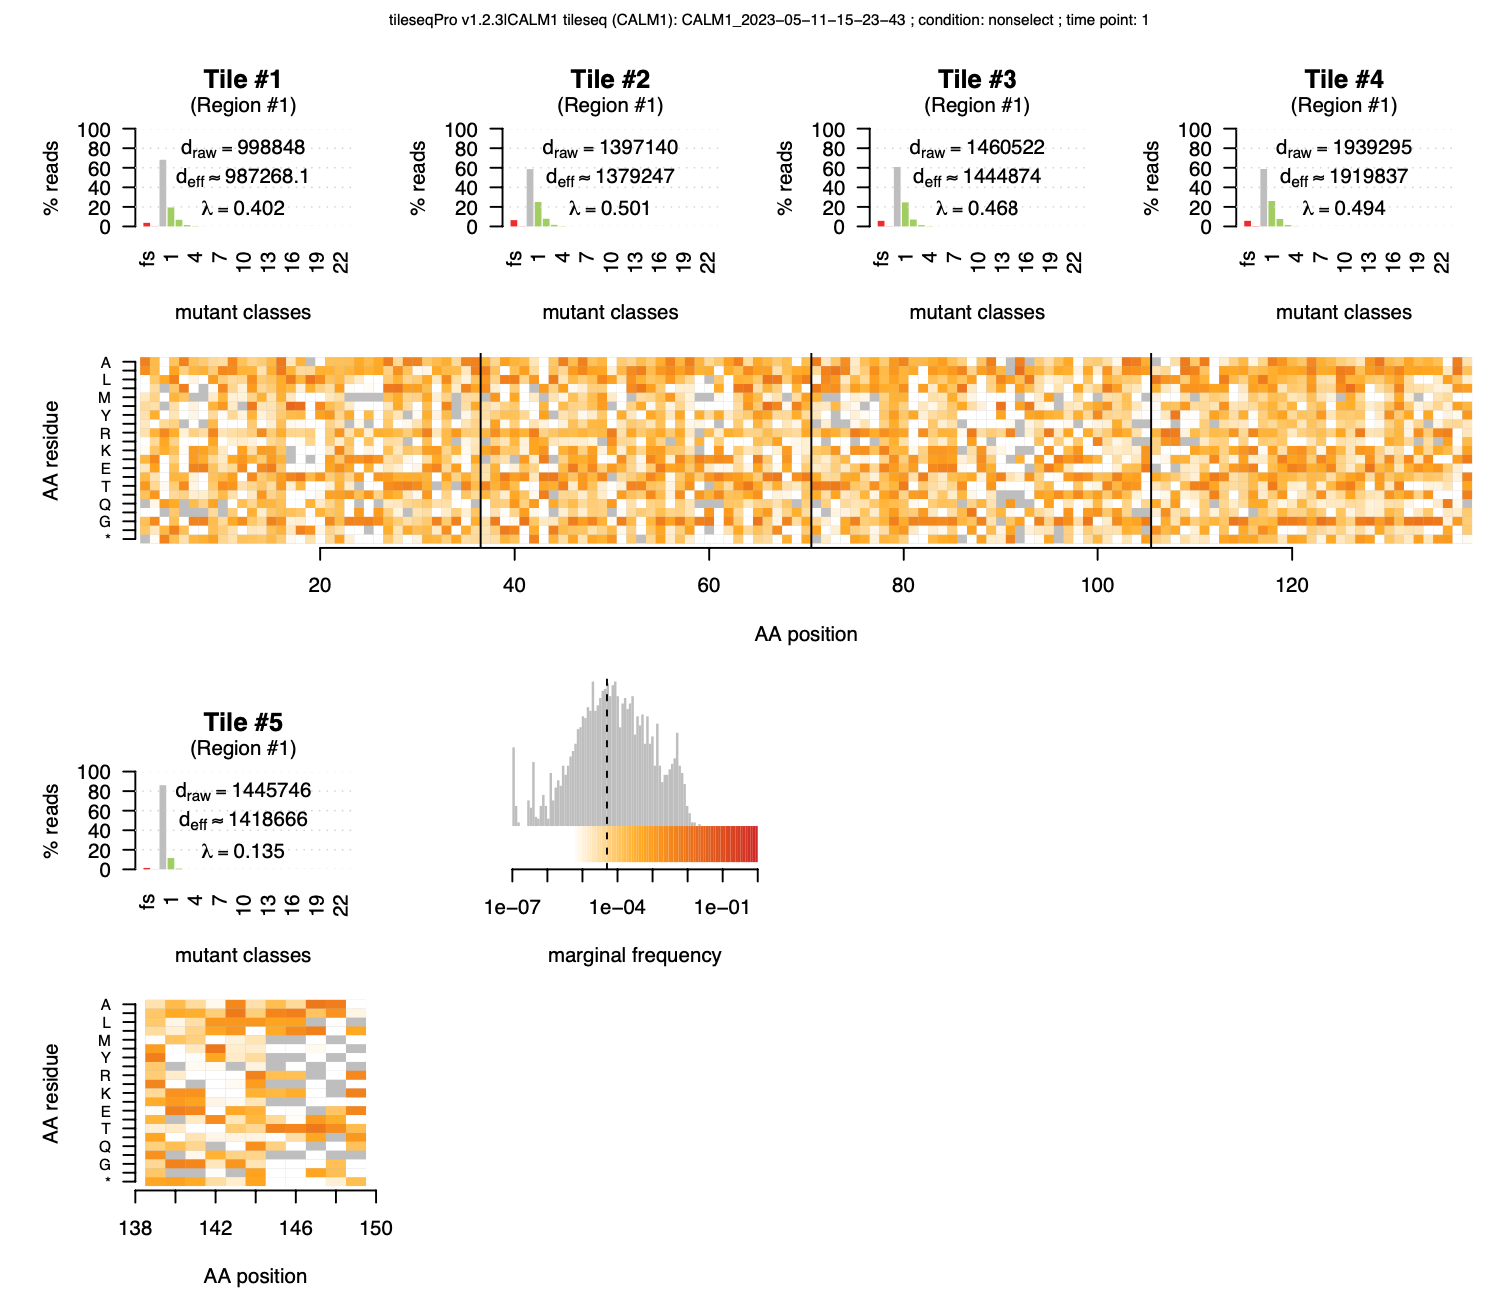
\includegraphics[width=.6\textwidth]{Figures/CALM1/coverage.png} }}%
    \qquad
    \subfloat[\centering Extrapolation for region 1]{{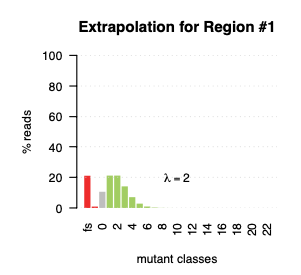
\includegraphics[width=.3\textwidth]{Figures/CALM1/extrapolation_CALM1.png} }}%
    \caption{The coverage heatmap and an extrapolation of the number of variants per clone for Region 1 for the re-calculated CALM1 map. The heatmap shows marginal frequencies for each amino acid change. Lambda refers to the mean of the best fitting Poisson distribution of the number of variants observed per read.}%a
    \label{fig:heatmap_CALM1}%
\end{figure}

% filtering CALM1
\begin{figure}[H]%
    \centering
    \subfloat[\centering $\log(\phi)$ bias plot]{{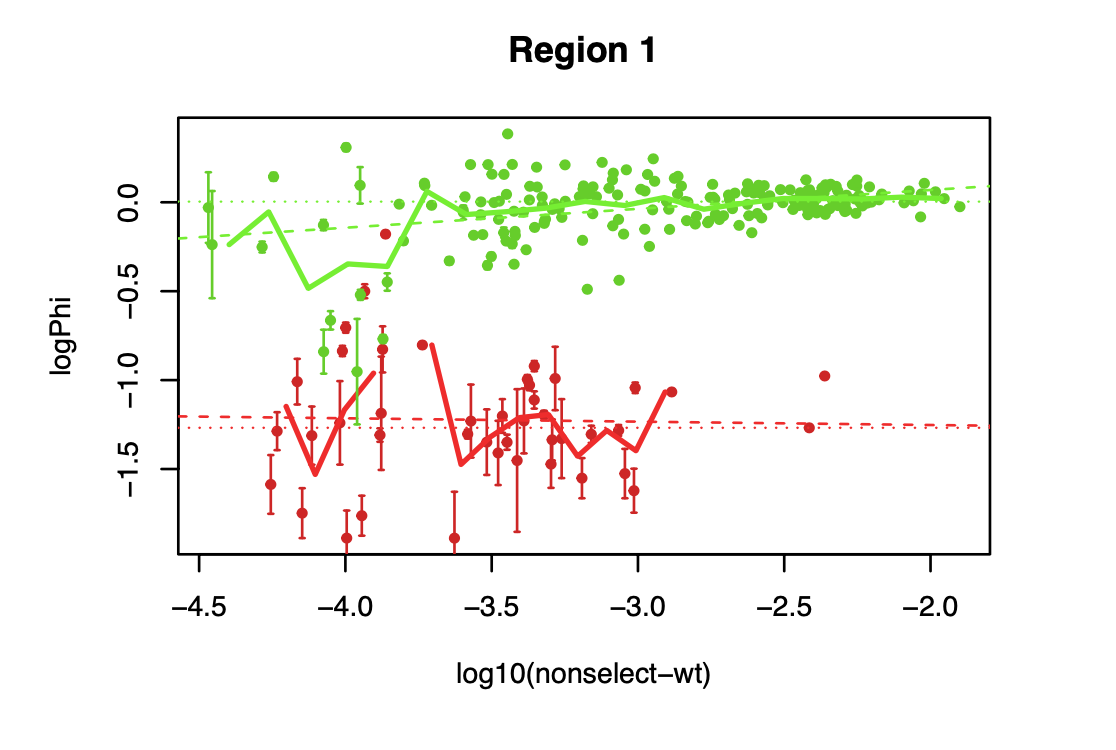
\includegraphics[width=.45\textwidth]{Figures/CALM1/logphi_bias.png} }}%
    \qquad
    \subfloat[\centering filtering breakdown]{{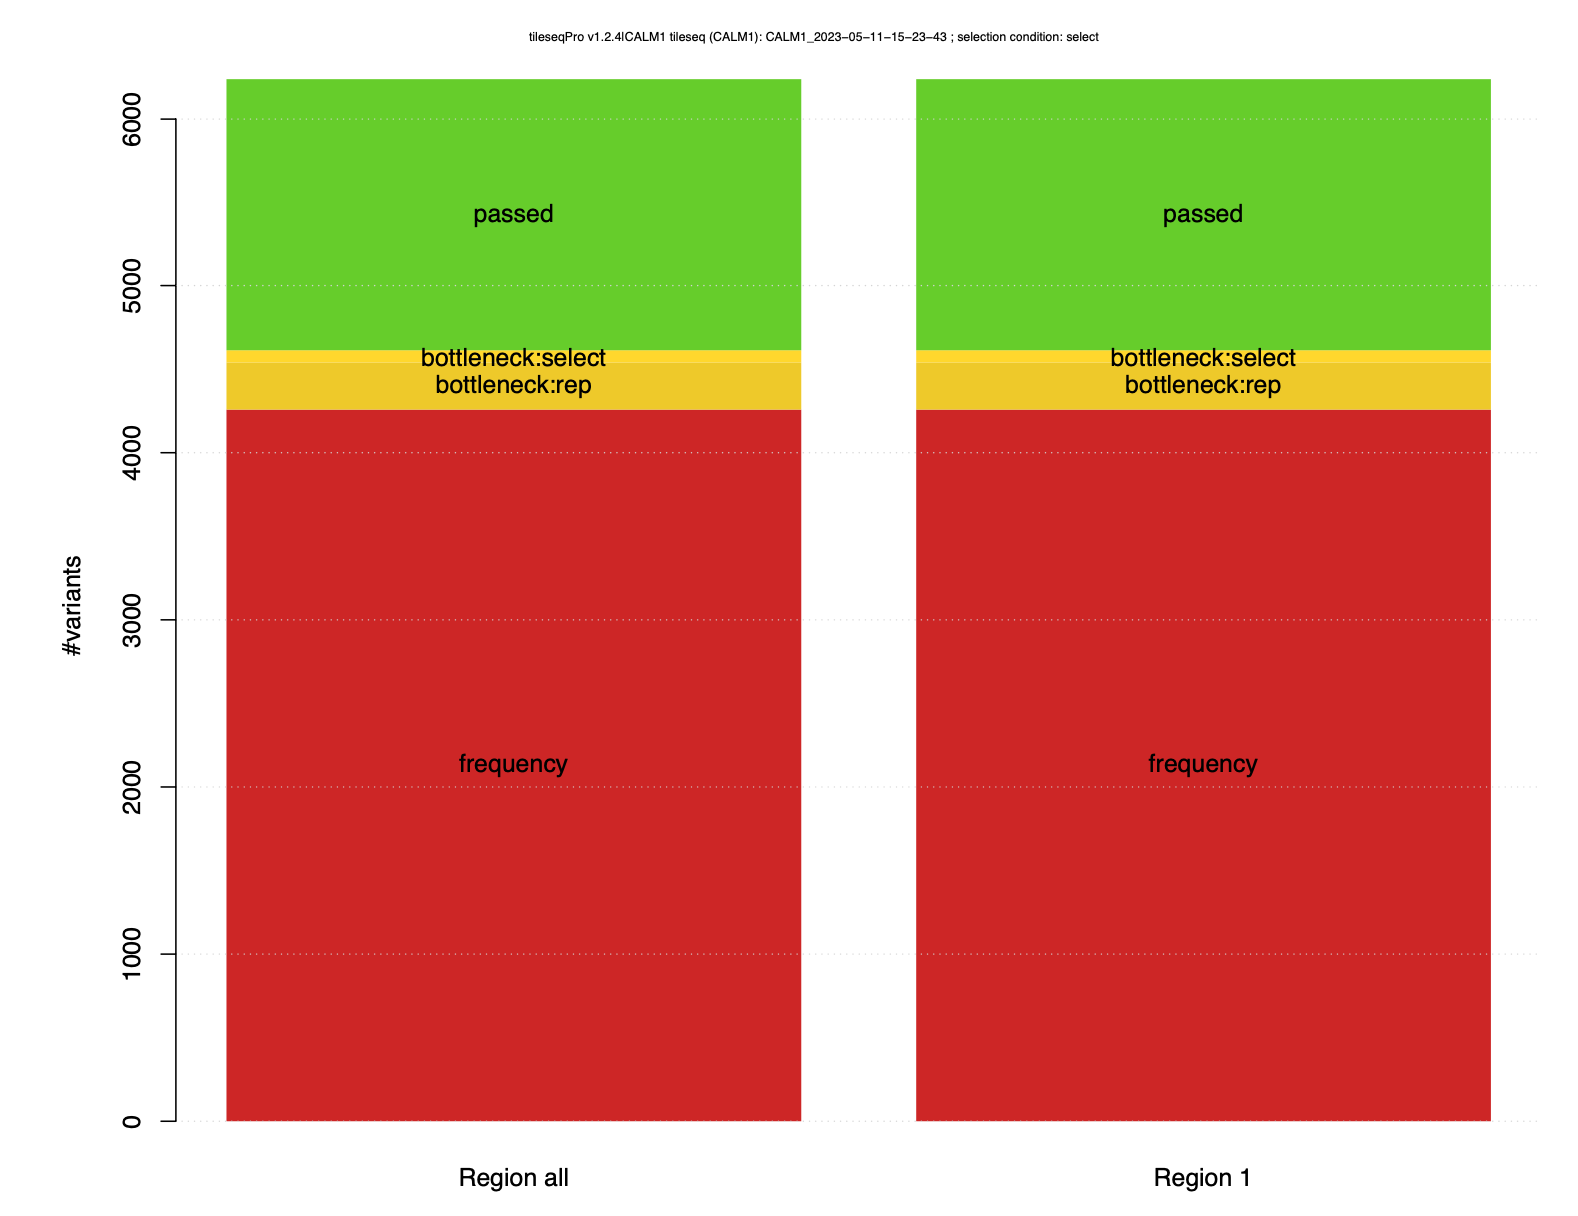
\includegraphics[width=.45\textwidth]{Figures/CALM1/filtering.png} }}%
    \caption{The $log(\phi)$ bias plot and the filtering breakdown bar plot for CALM1 map. The $log(\phi)$ bias plot illustrates how the $\log(\phi)$ values of synonymous(green) and nonsense(red) variants changing as the read frequency cutoff increasing. The filtering breakdown plot show the number of CALM1 variants in region 1 that were subjected to individual filters.}%
    \label{fig:filtering_CALM1}%
\end{figure}


% CALM1 se boxplots
\begin{figure}[H]
    \centering
    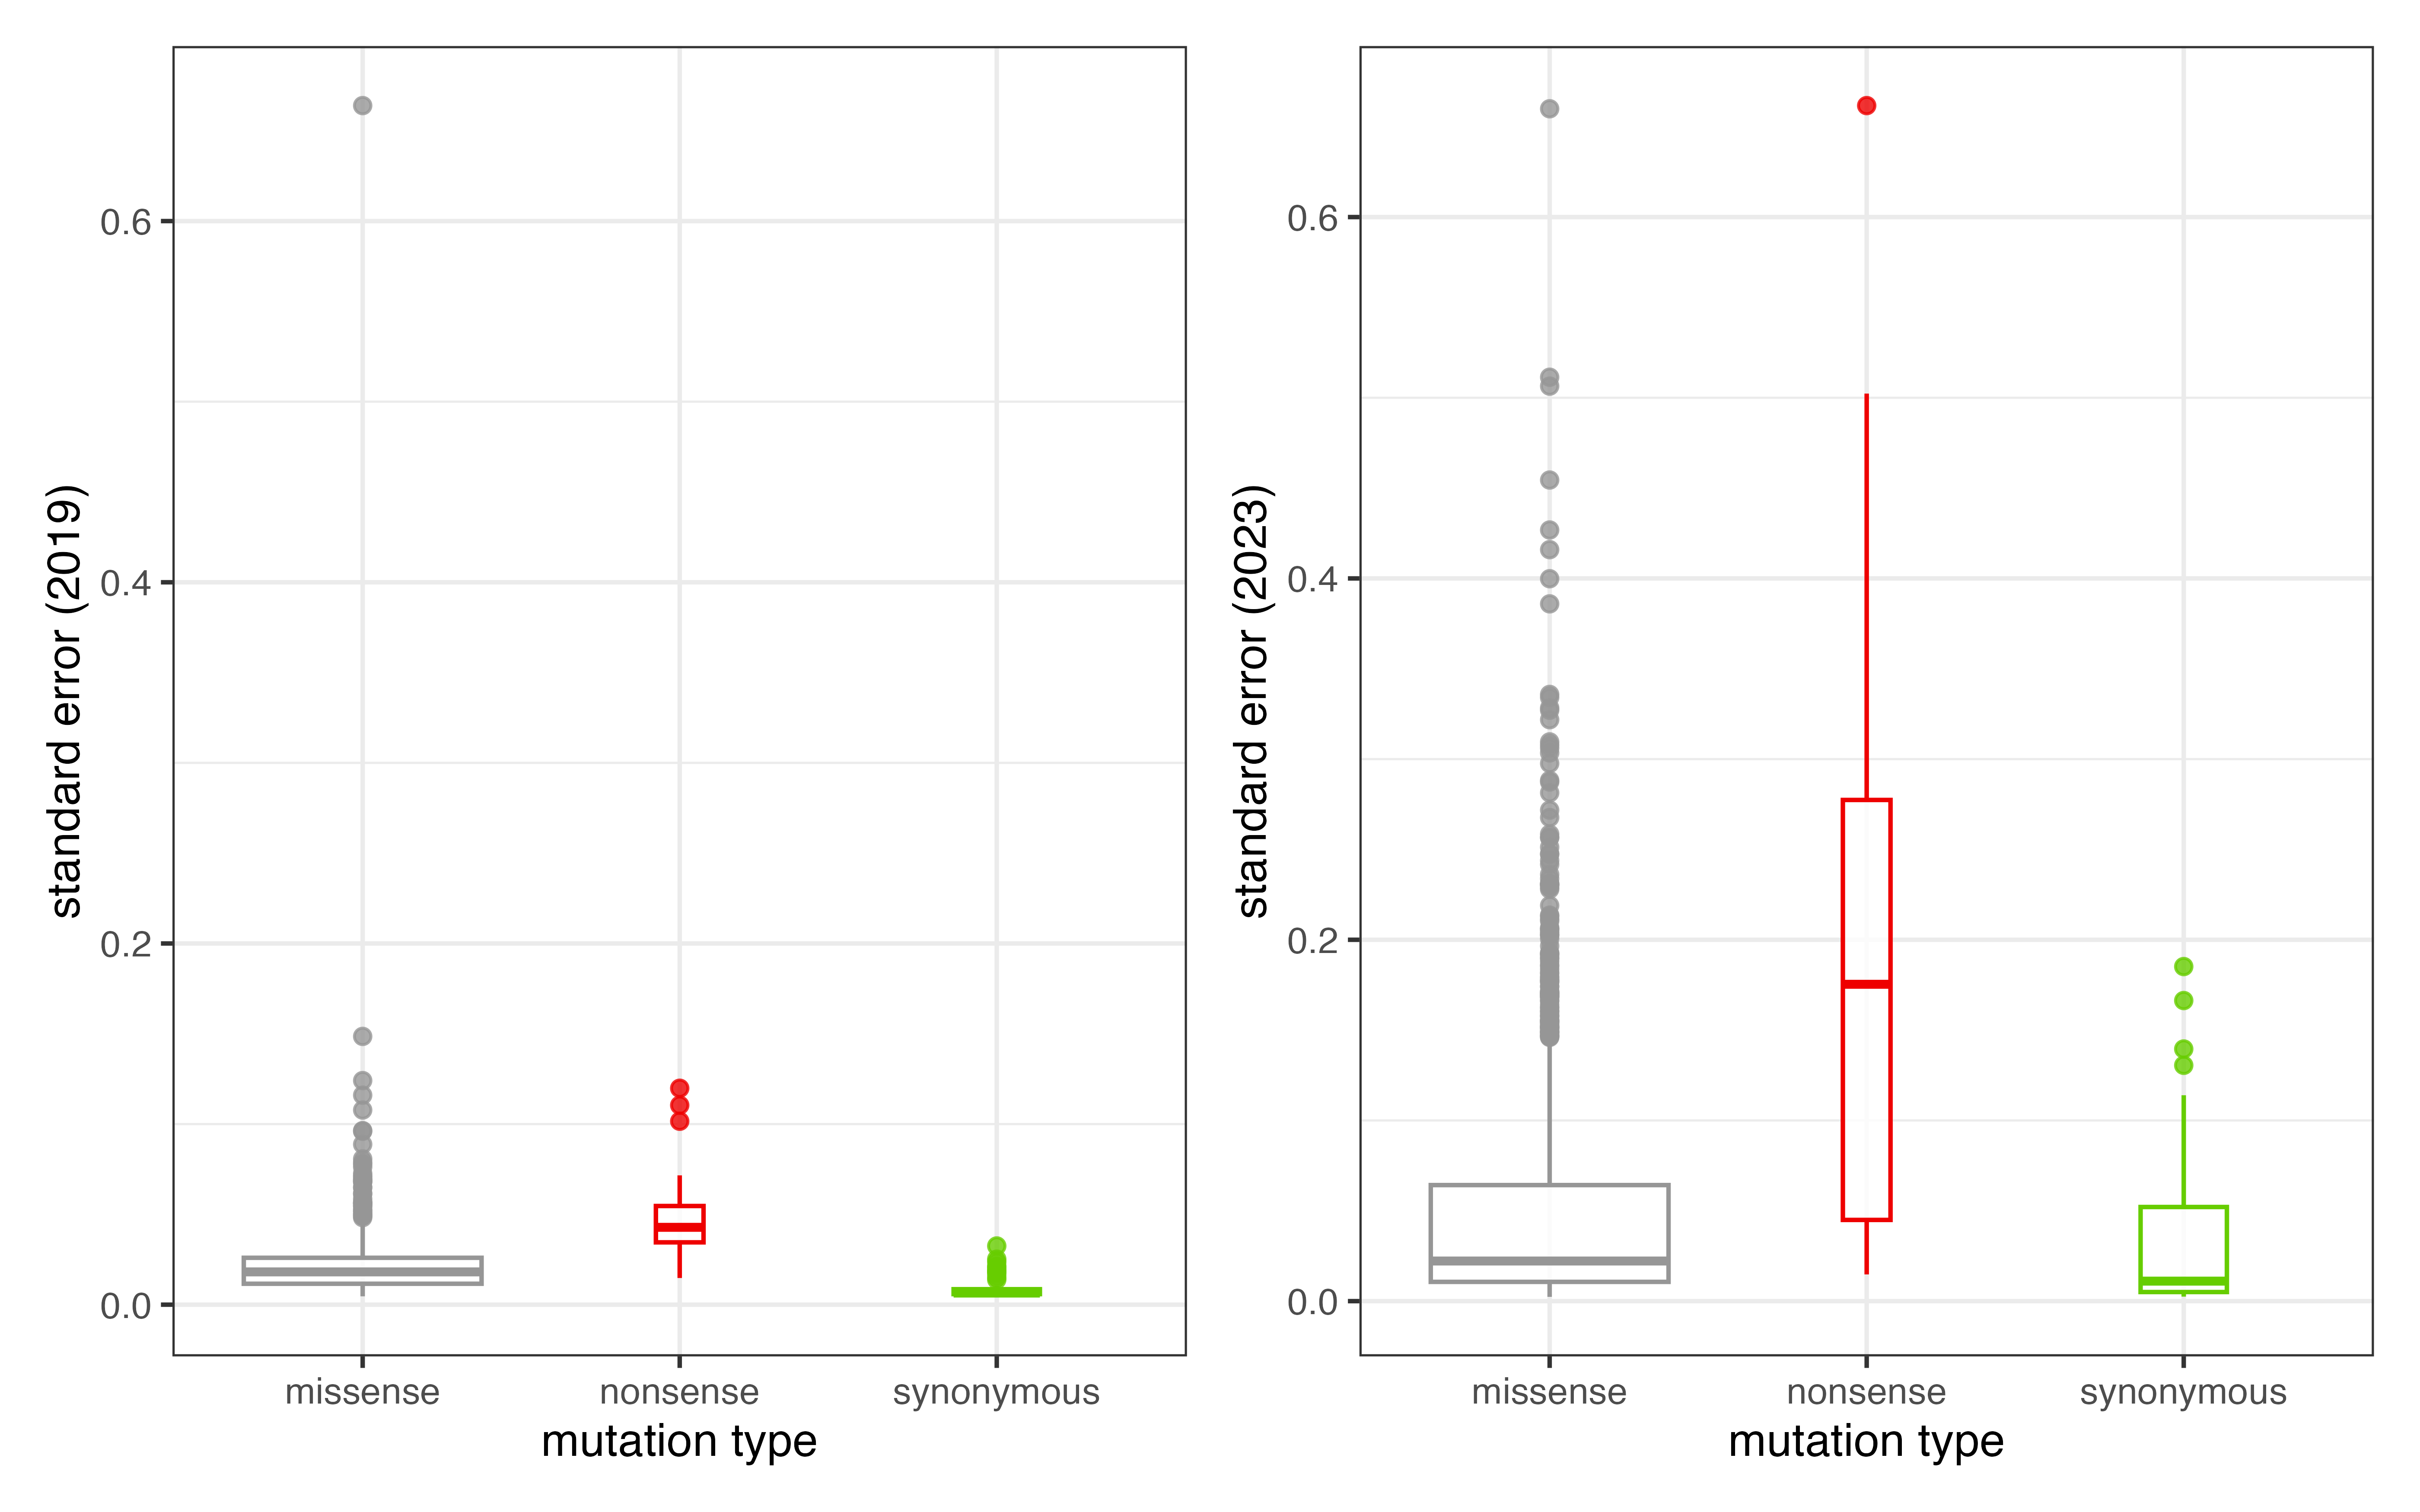
\includegraphics[width =.8\textwidth]{Figures/CALM1/se_boxplot.png}
    \caption{The distribution of standard error of new and old fitness scores (CALM1).}
    \label{fig:se boxplot CALM1}
\end{figure}


% CALM1 Score Comparison
\begin{figure}[H]%
    \centering
    \subfloat[\centering ]{{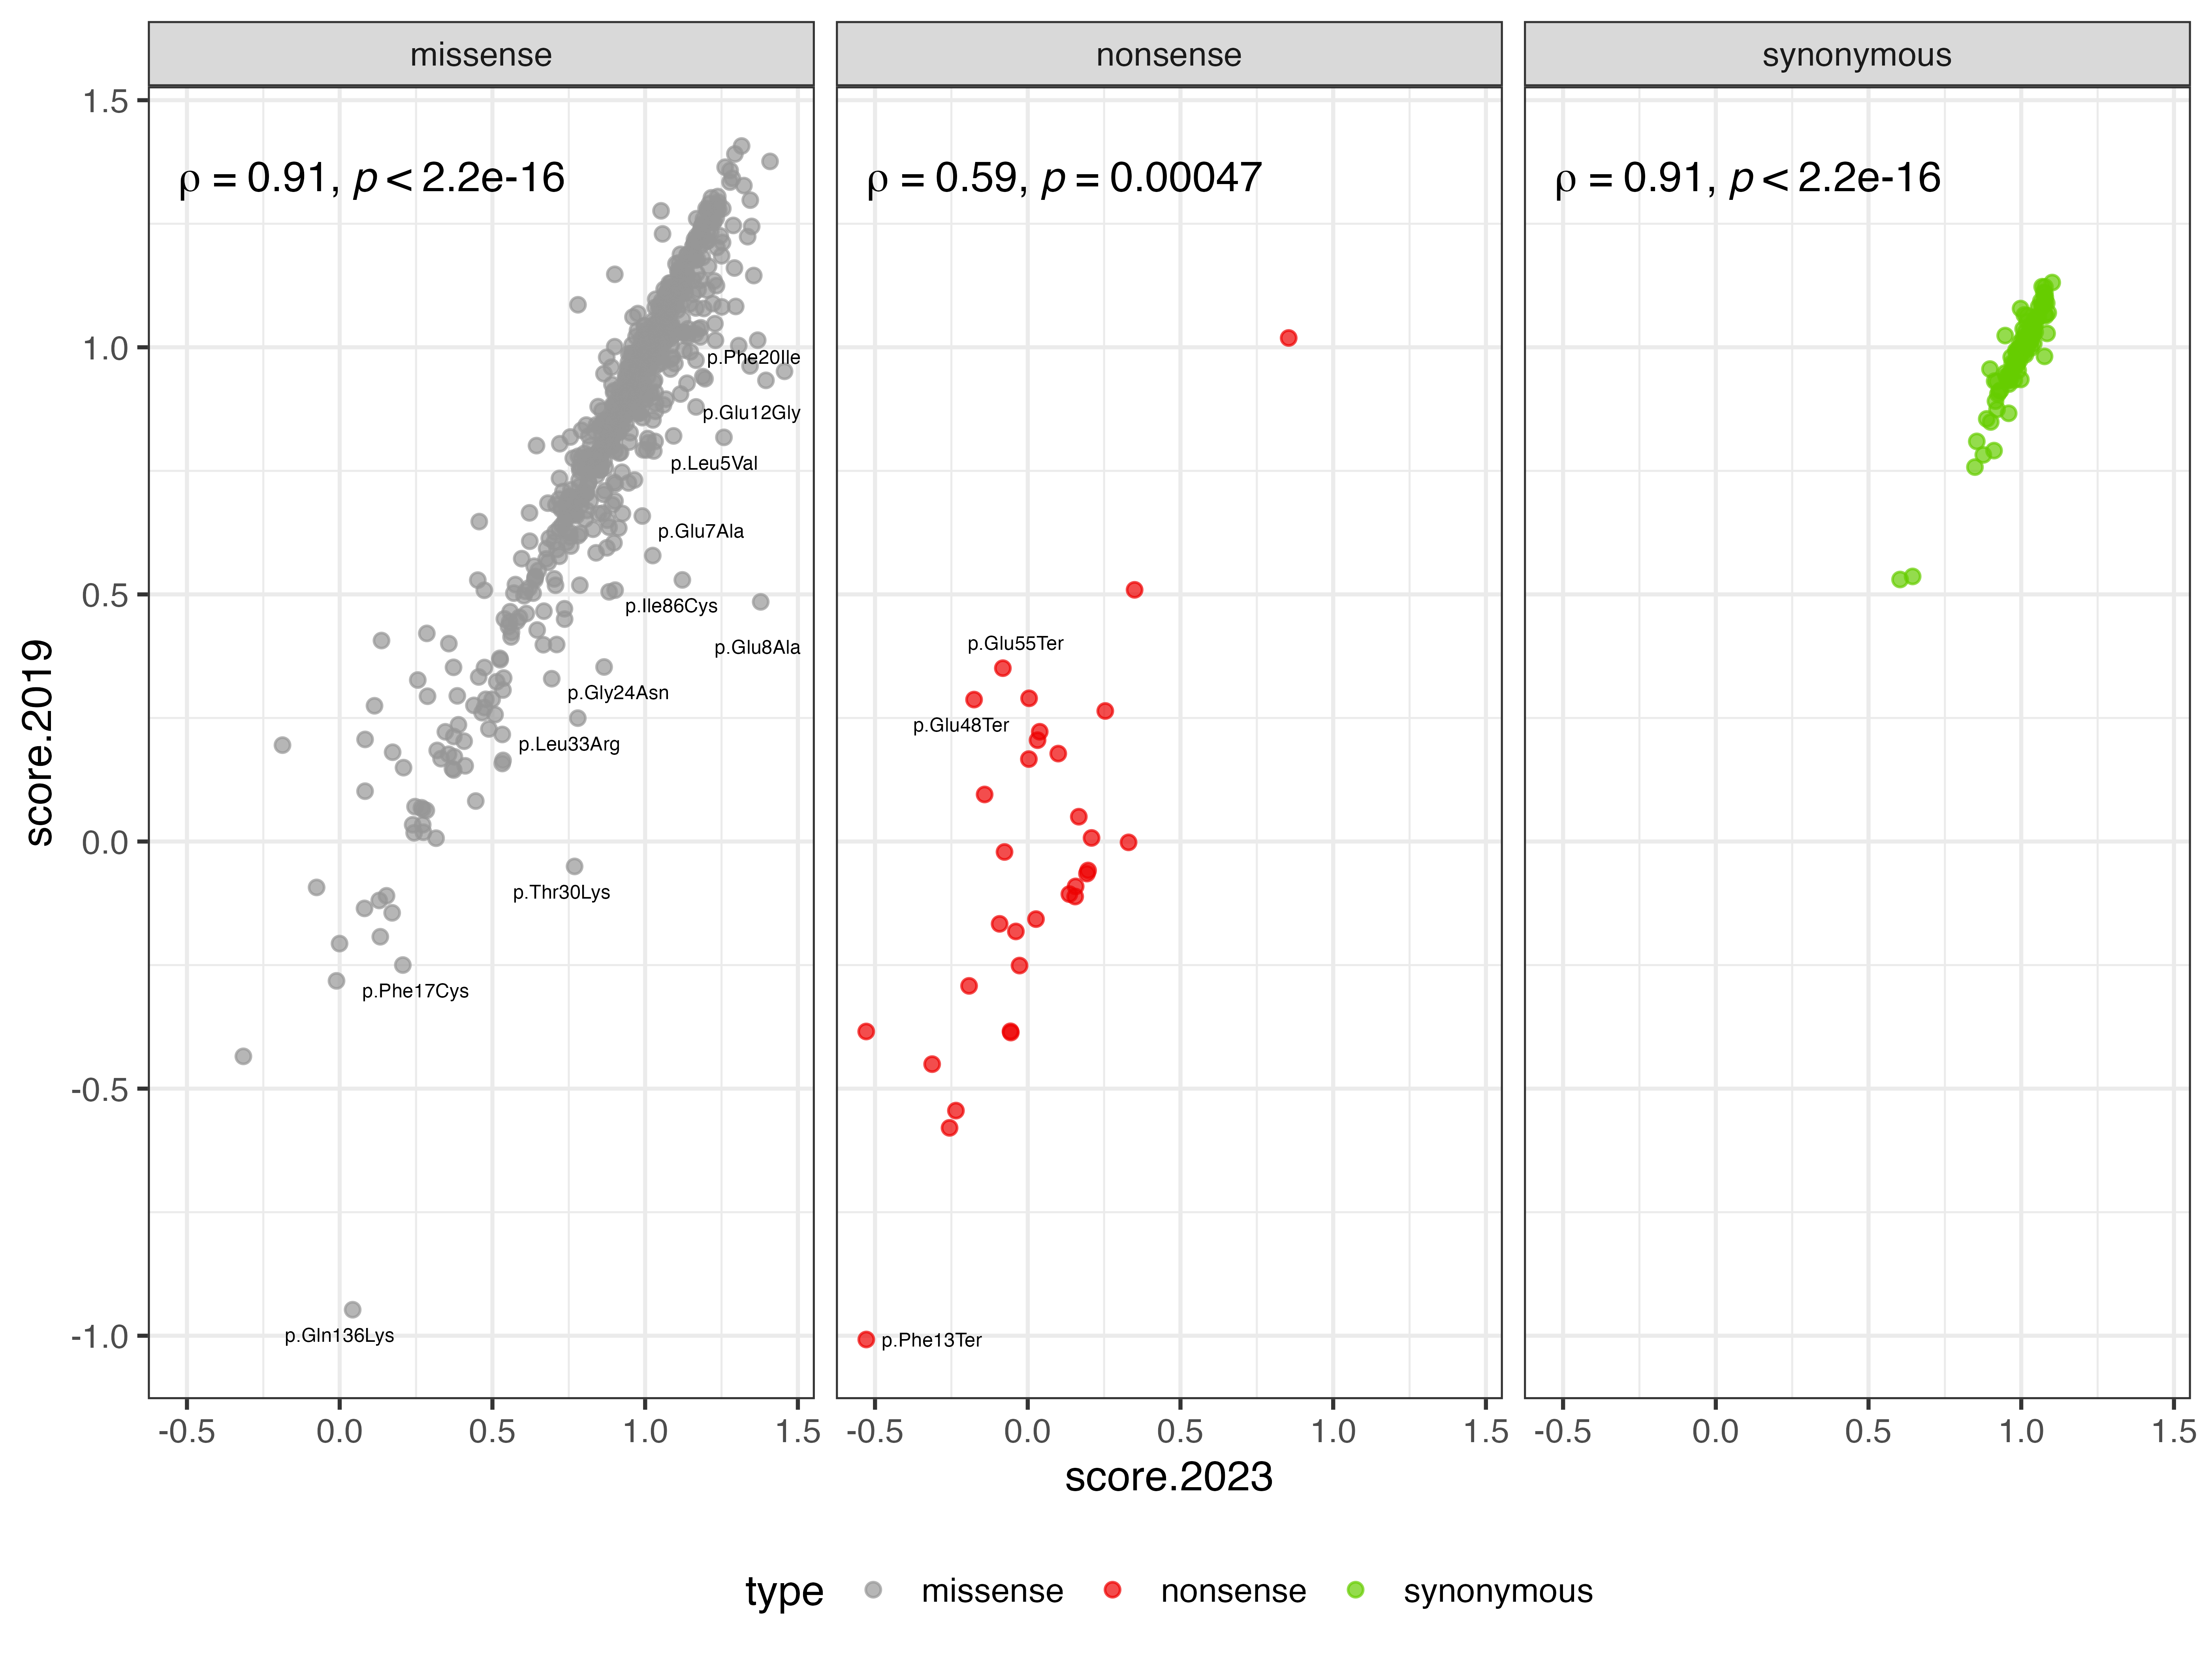
\includegraphics[width=.57\textwidth]{Figures/CALM1/comparison_mutation.png} }}%
    \qquad
    \subfloat[\centering ]{{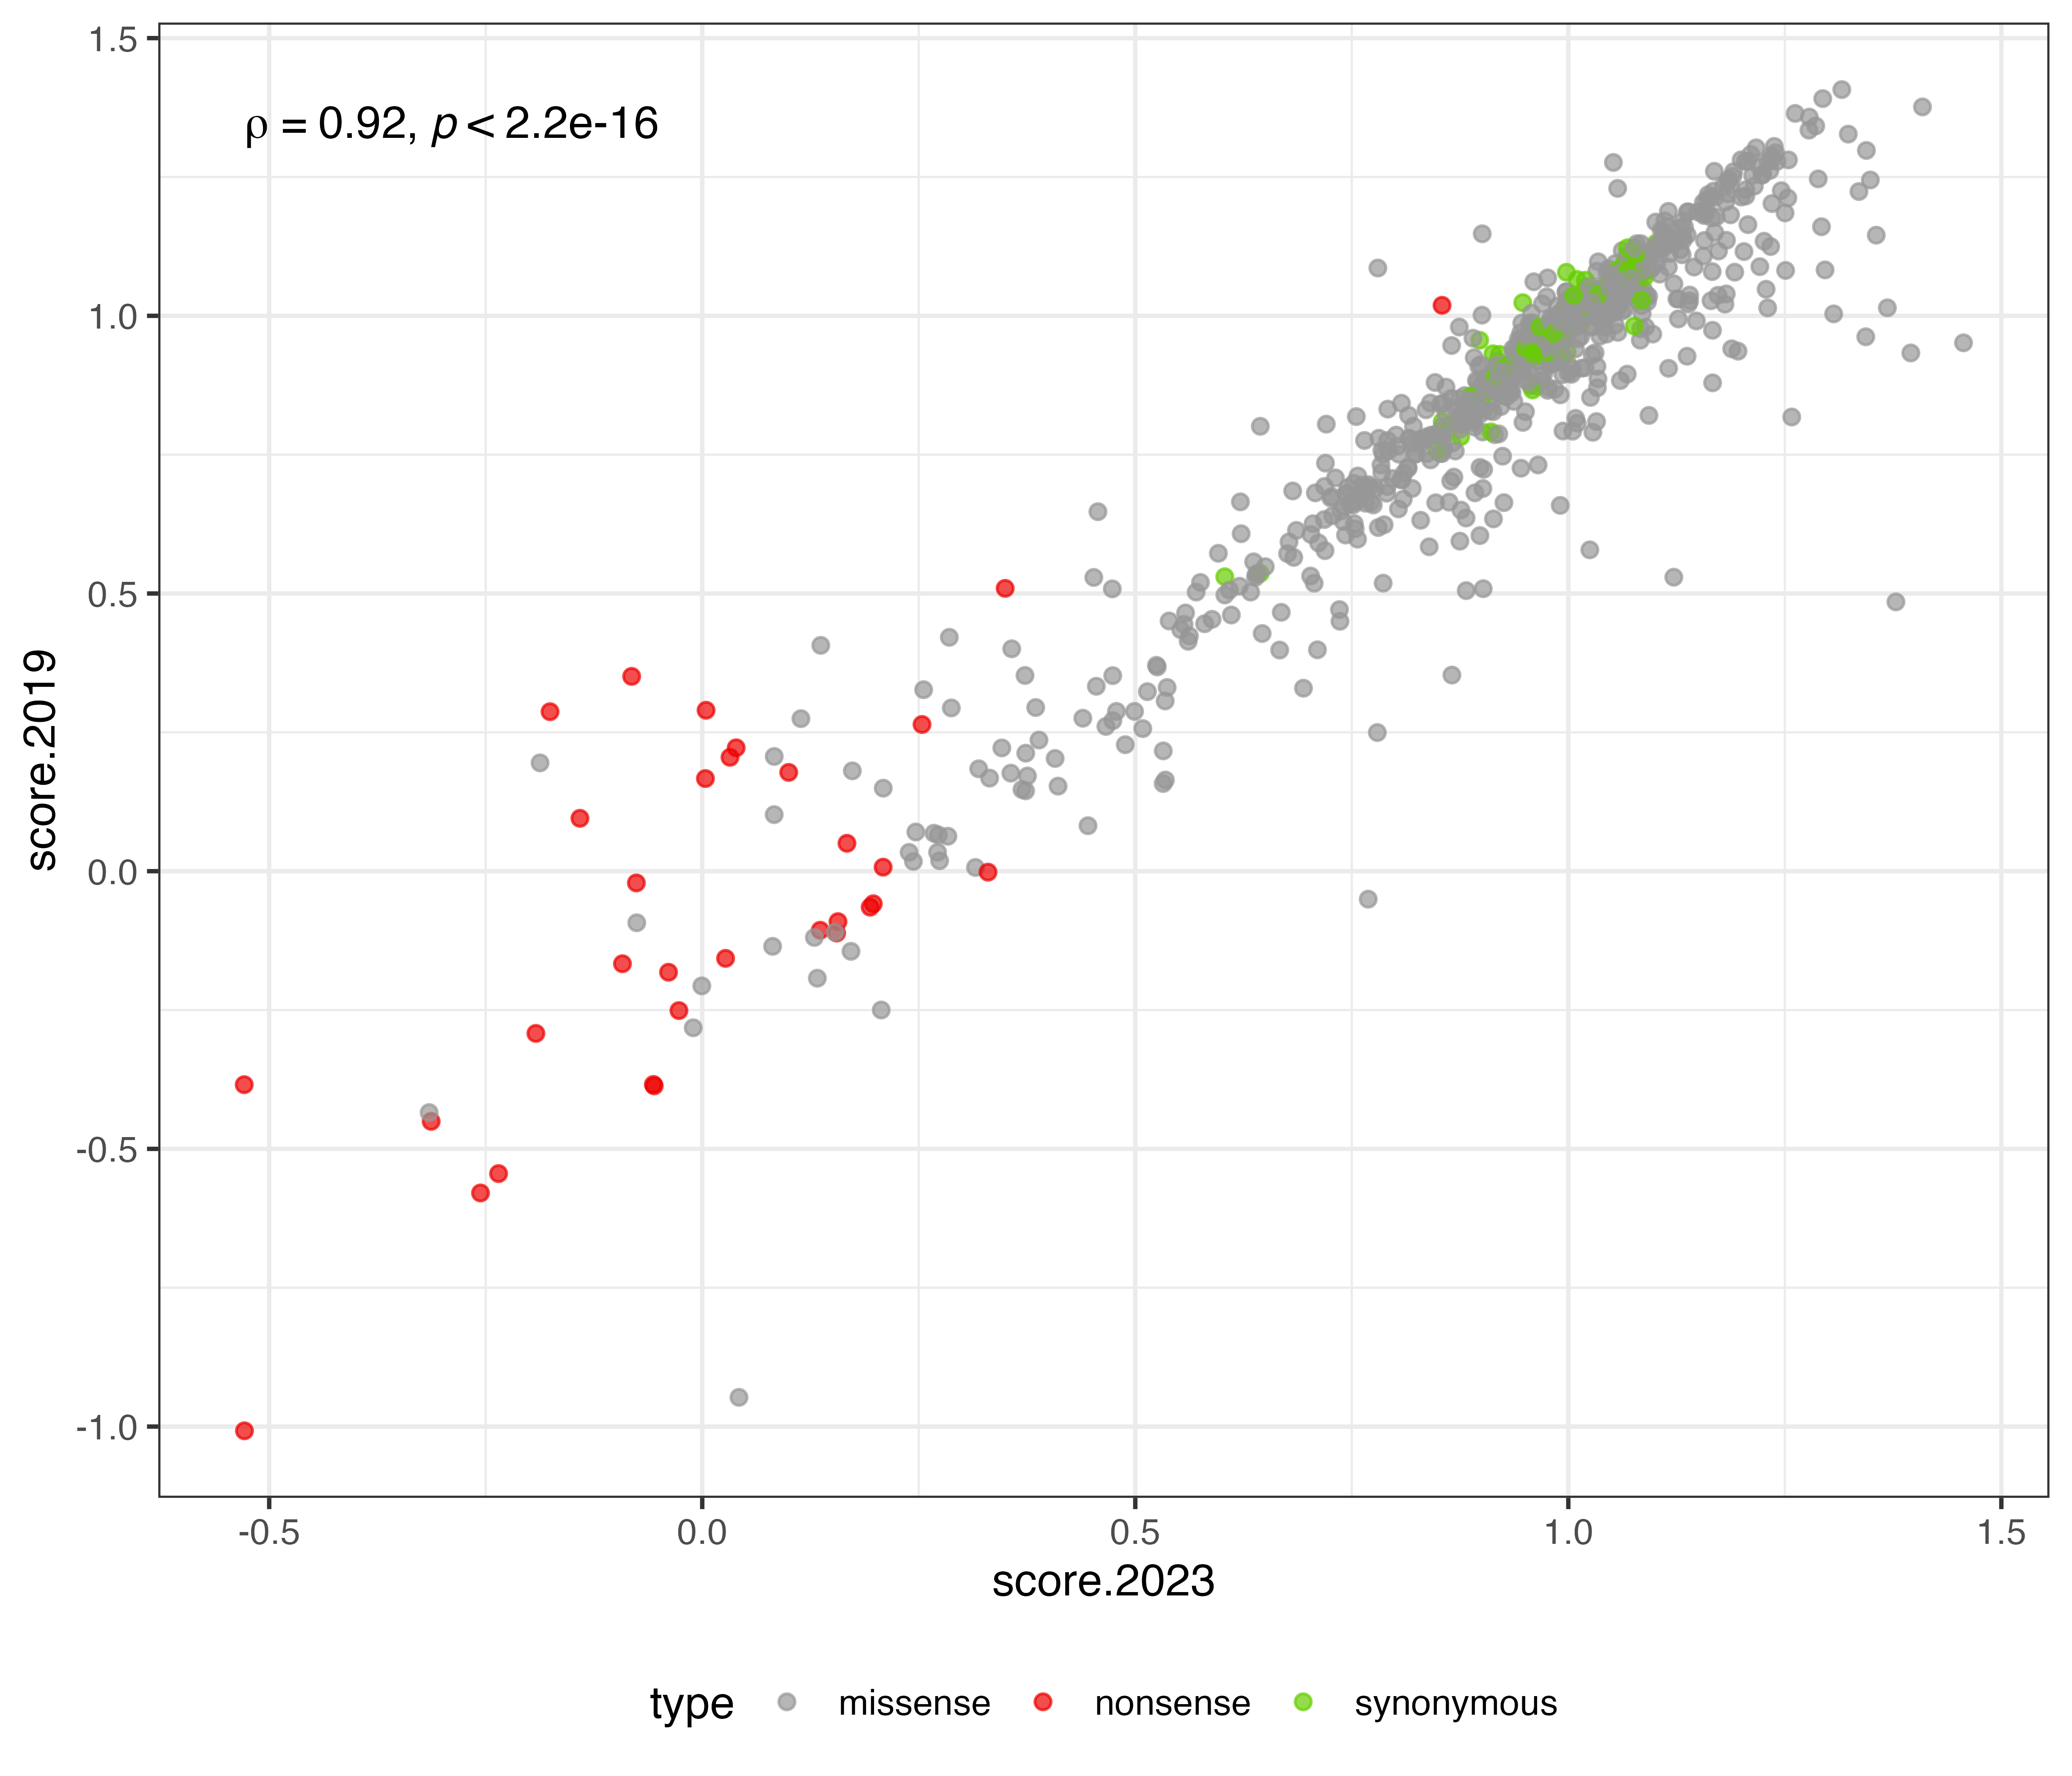
\includegraphics[width=.57\textwidth]{Figures/CALM1/comparison_overall.png} }}%
    \qquad
    \subfloat[\centering ]{{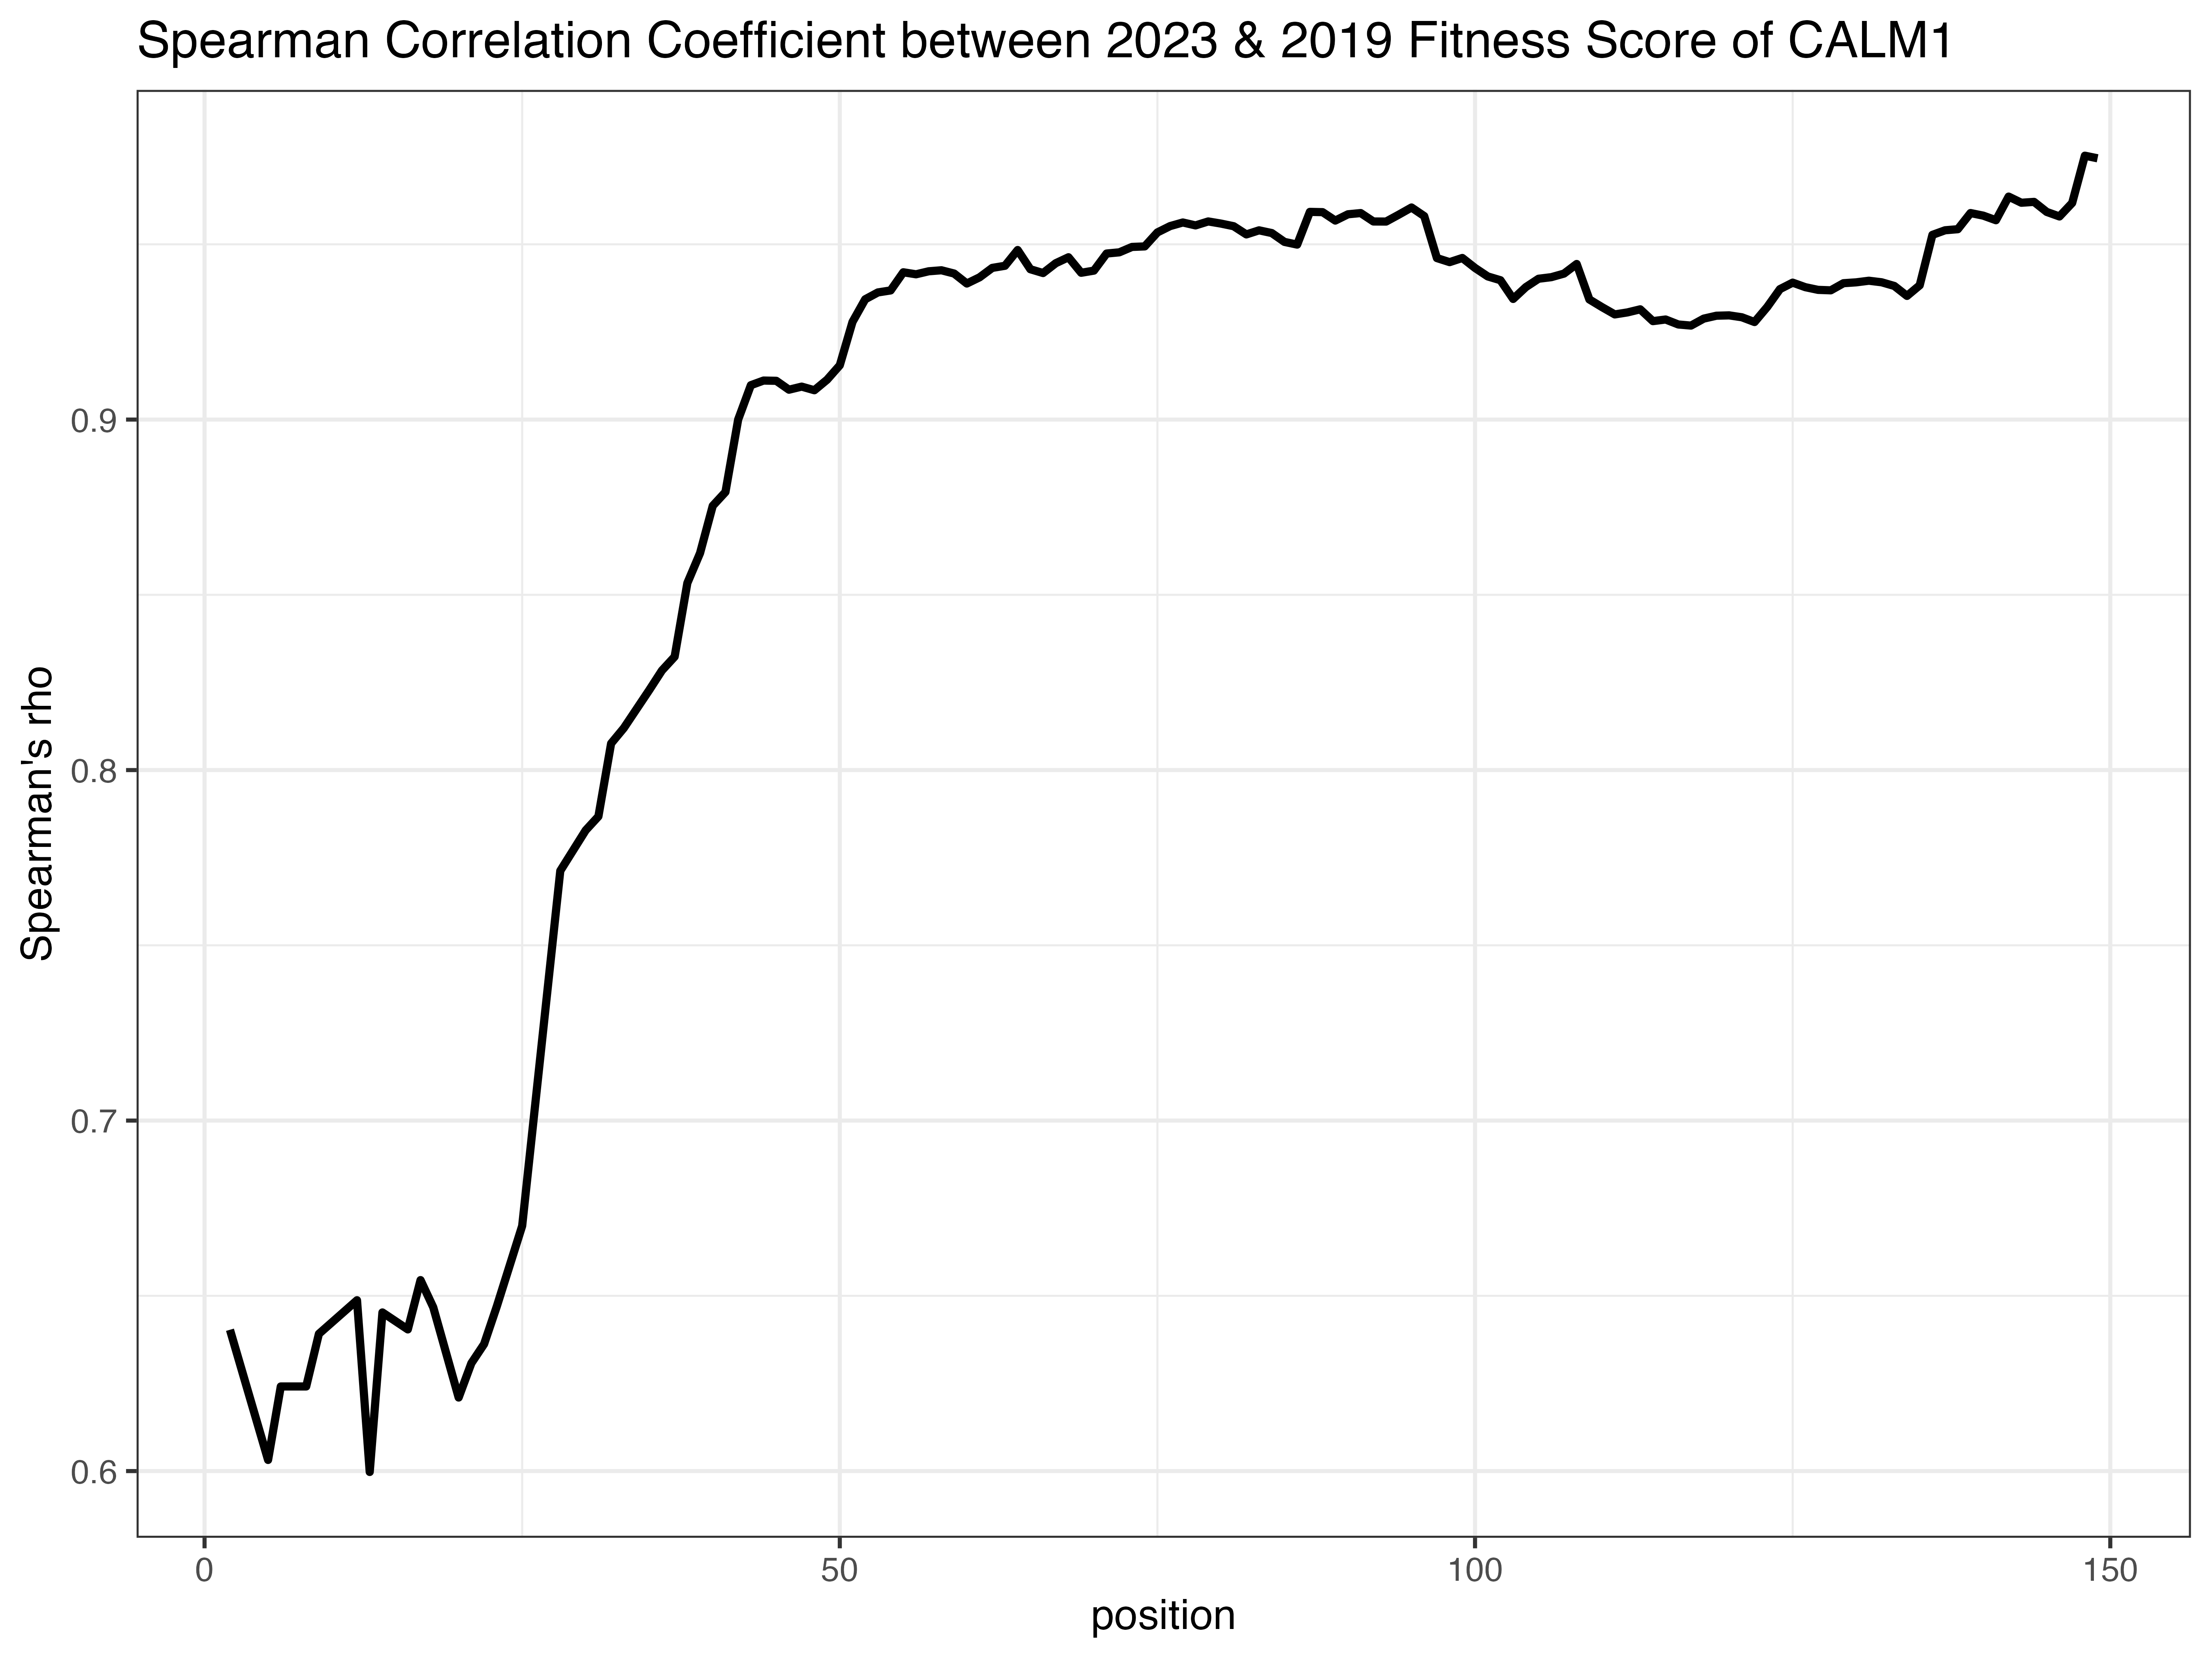
\includegraphics[width=.57\textwidth]{Figures/CALM1/score_rho.png} }}%
    \caption{(a) and (b) show the scatter plot of fitness scores for CALM1 generated by TileseqPro and Legacy pipelines, (c) is a line graph describing the change of Spearman's correlation between fitness scores along amino acid positions.}%
    \label{fig:scatter plot CALM1}%
\end{figure}



\subsection{MTHFR in A222V Background}
% coverage heatmap
\begin{figure}[H]%
    \centering
    \subfloat[\centering ]{{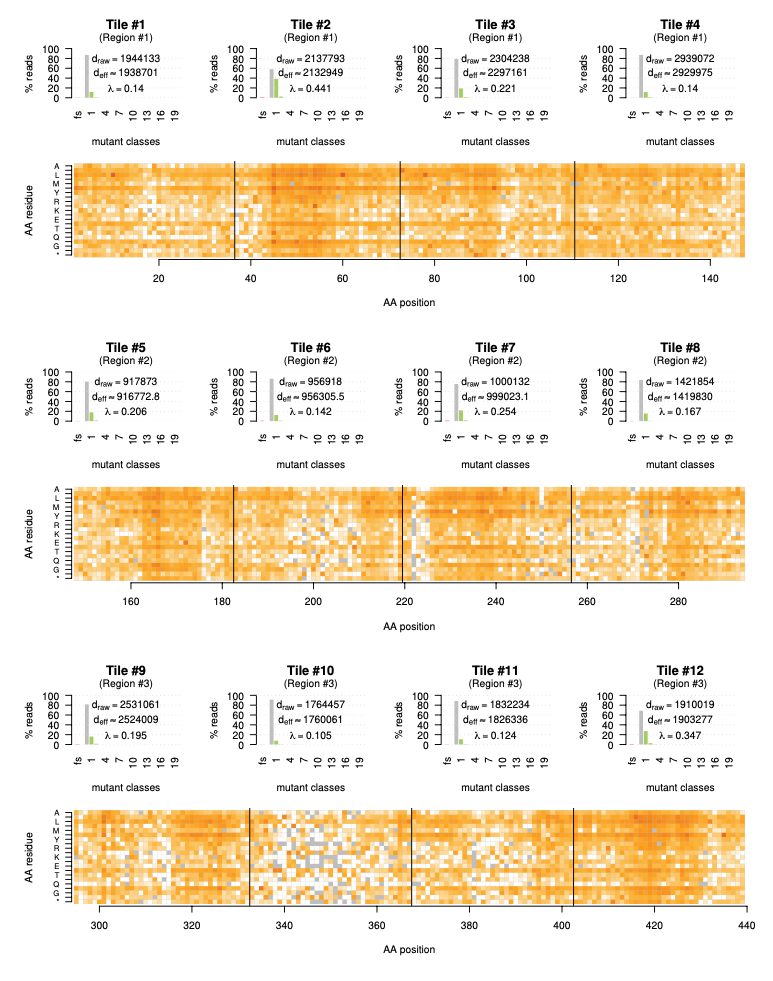
\includegraphics[width=.6\textwidth]{Figures/MTHFR/coverage_heatmap_nsNew.png} }}%
    \qquad
    \subfloat[\centering ]{{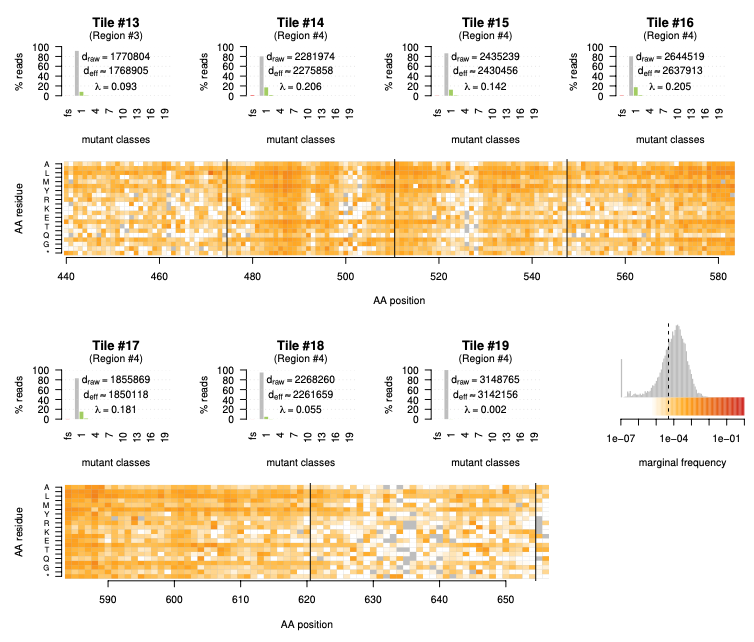
\includegraphics[width=.6\textwidth]{Figures/MTHFR/coverage_heatmap_nsNew_2.png} }}%
    \caption{(a) and (b) show the coverage heatmaps for MTHFR in Ala222Val Background.}%
    \label{fig:coverage MTHFR}%
\end{figure}





% extrapolation for all region
\begin{figure}[H]
    \centering
    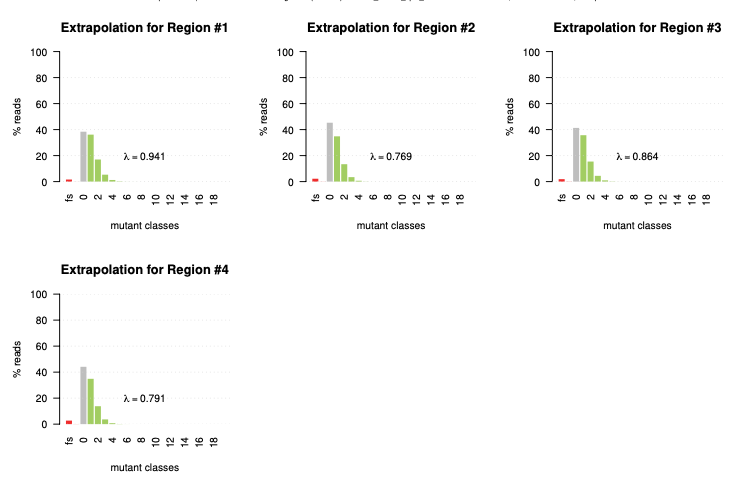
\includegraphics[width =.8\textwidth]{Figures/MTHFR/extrapolation_nsNew.png}
    \caption{The extrapolation of the number of variants per clone ($\lambda$) for Region 1 to 4 for the re-calculated MTHFR in A222V background}
    \label{fig: extrapolation for all region}
\end{figure}

% logphi bias plot for all folate concentrations
\begin{figure}[H]%
    \centering
    \subfloat[\centering f12AV]{{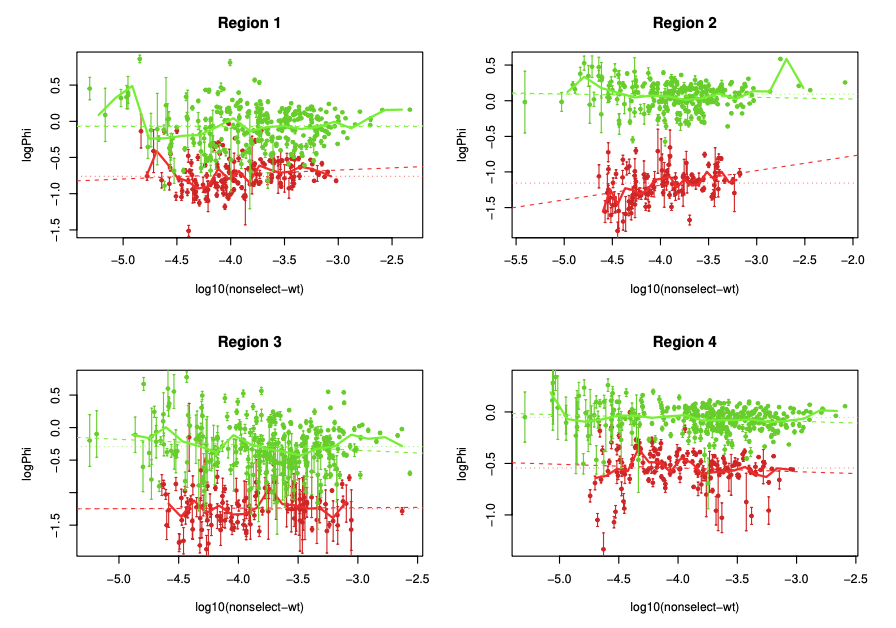
\includegraphics[width=.45\textwidth]{Figures/MTHFR/f12AV_logphi_bias.png} }}%
    \qquad
    \subfloat[\centering f25AV]{{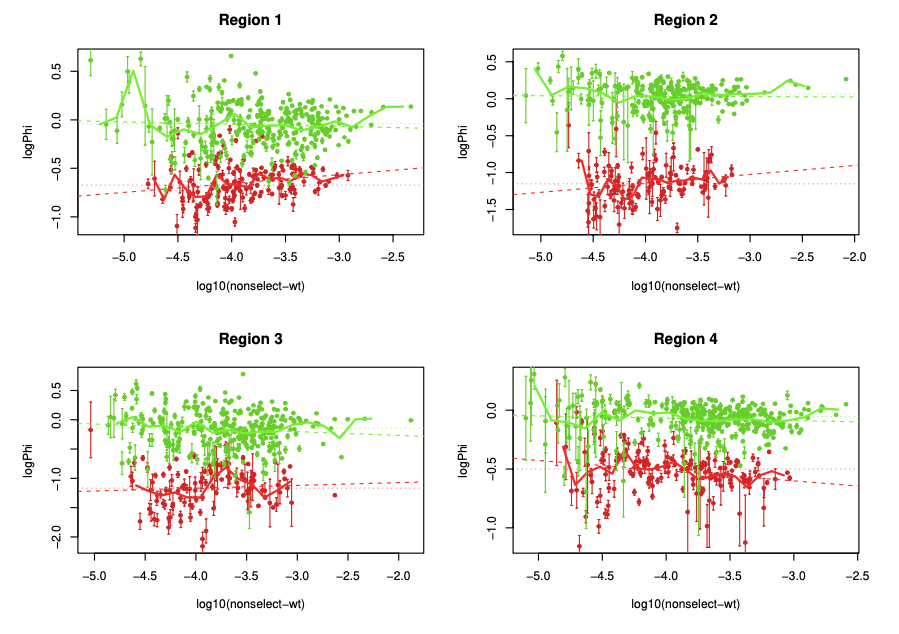
\includegraphics[width=.45\textwidth]{Figures/MTHFR/f25AV_logphi_bias.png} }}%
    \qquad
    \subfloat[\centering f100AV]{{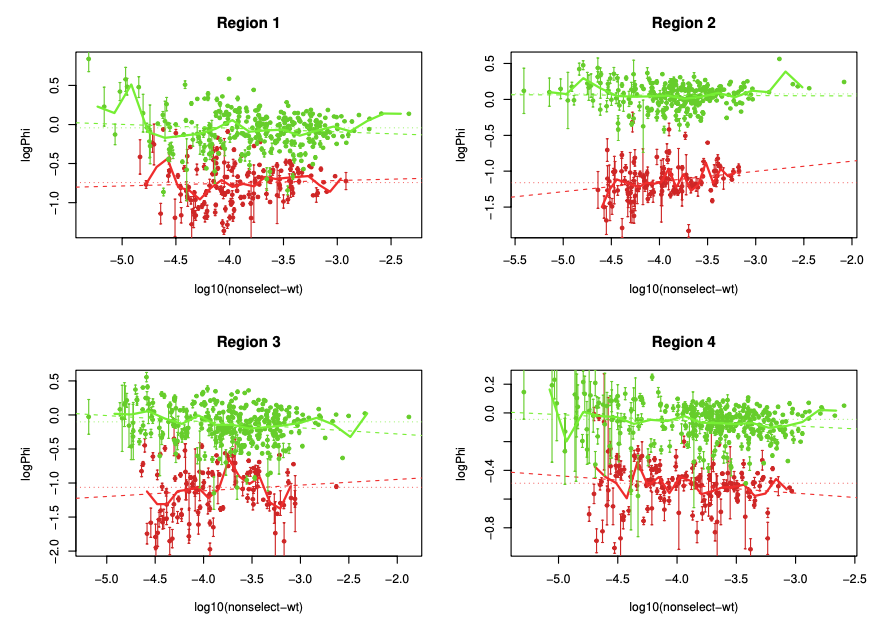
\includegraphics[width=.45\textwidth]{Figures/MTHFR/f100AV_logphi_bias.png} }}%
    \qquad
    \subfloat[\centering f200AV]{{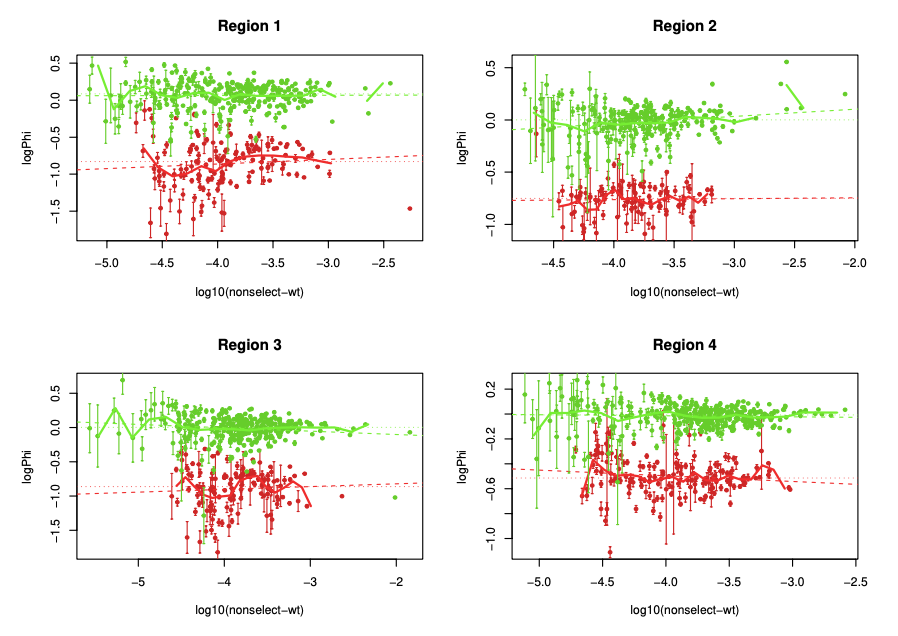
\includegraphics[width=.45\textwidth]{Figures/MTHFR/f200AV_logphi_bias.png} }}%
    \caption{The distribution of nonsense and synonymous MTHFR variants enrichment ratio ($log(\phi)$) relative to marginal frequency thresholds at different folate concentrations}%
    \label{fig:logphi bias MTHFR}%
\end{figure}

% filtering breakdown
\begin{figure}[H]%
    \centering
    \subfloat[\centering f12AV]{{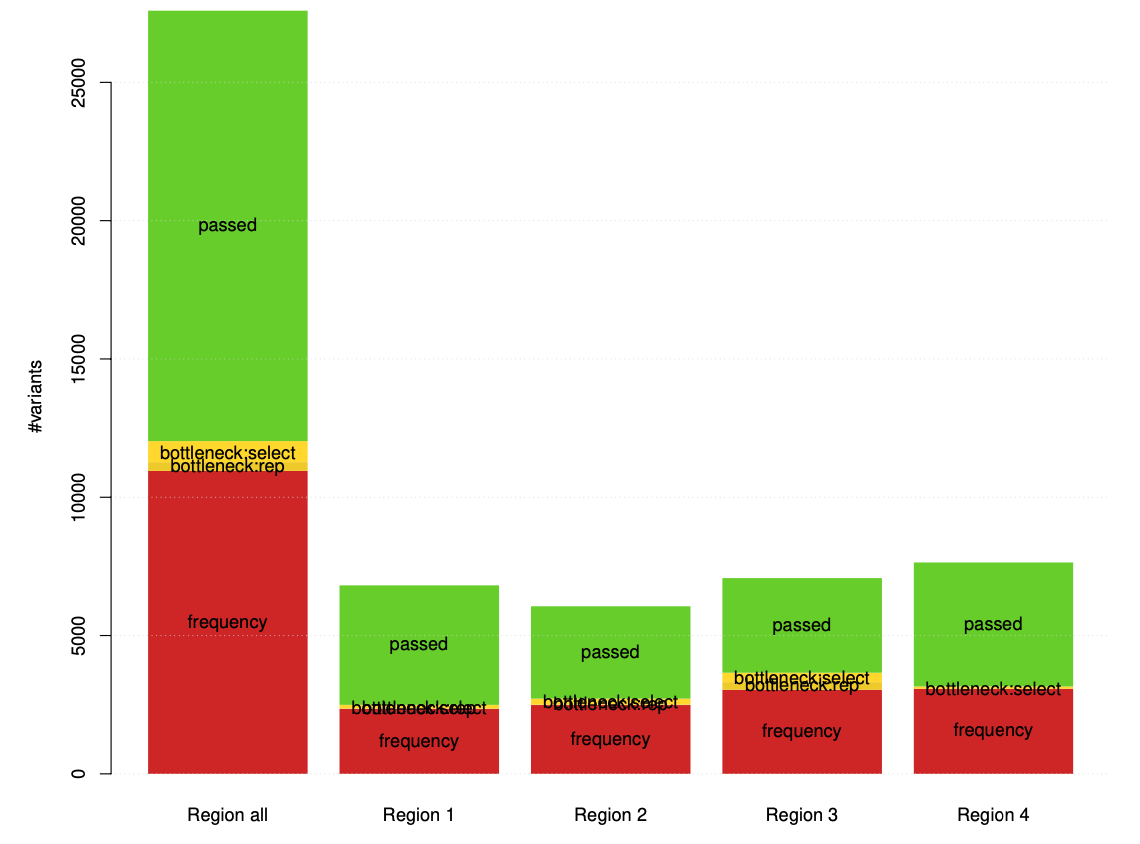
\includegraphics[width=.45\textwidth]{Figures/MTHFR/f12AV_filtering.png} }}%
    \qquad
    \subfloat[\centering f25AV]{{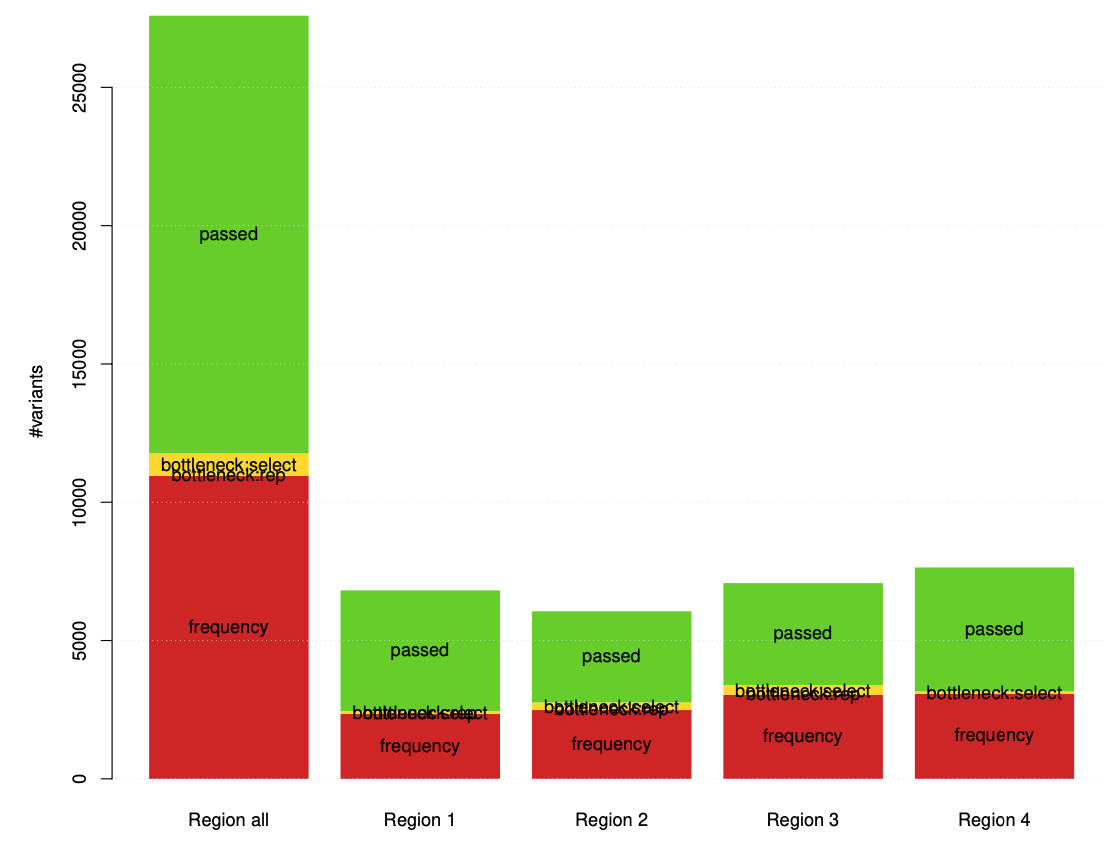
\includegraphics[width=.45\textwidth]{Figures/MTHFR/f25AV_filtering.png} }}%
    \qquad
    \subfloat[\centering f100AV]{{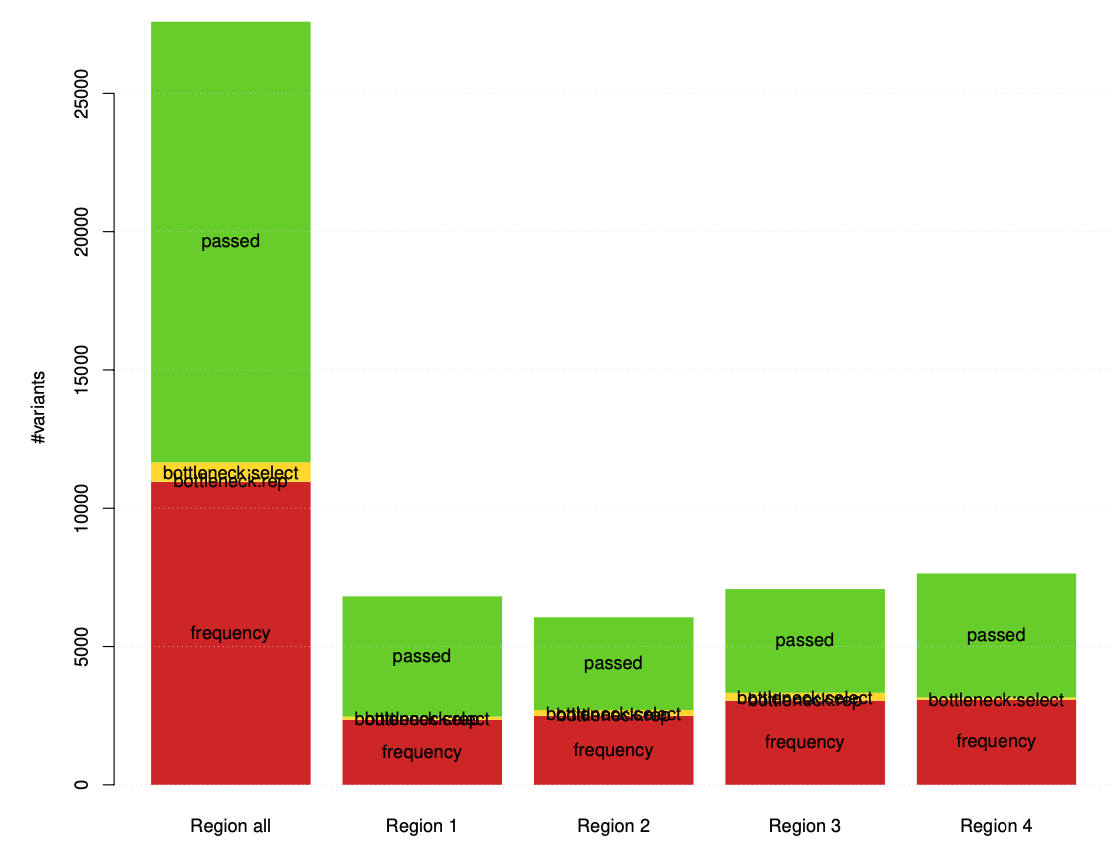
\includegraphics[width=.45\textwidth]{Figures/MTHFR/f100AV_filtering.png} }}%
    \qquad
    \subfloat[\centering f200AV]{{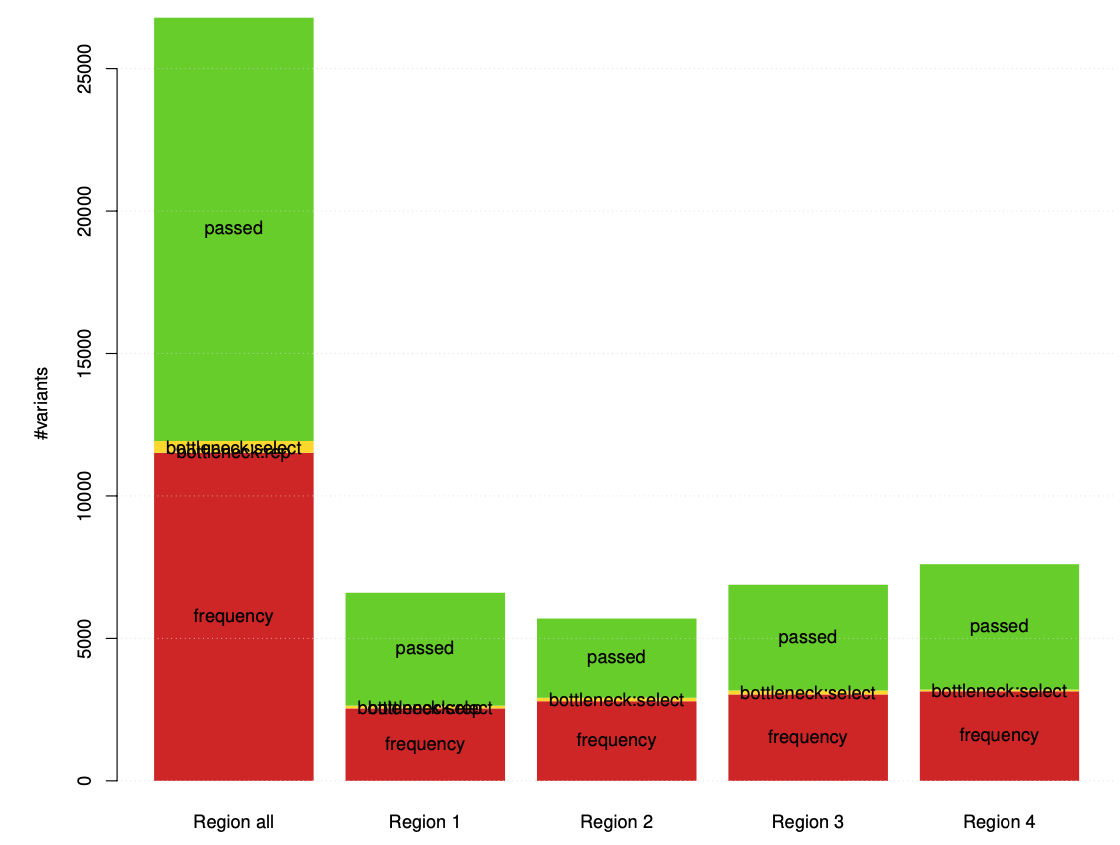
\includegraphics[width=.45\textwidth]{Figures/MTHFR/f200AV_filtering.png} }}%
    \caption{The filtering breakdown for MTHFR variants in A222V background at different folate concentrations.}%
    \label{fig:MTHFR filtering breakdown}%
\end{figure}









% LLR?
\begin{figure}[H]%
    \centering
    \subfloat[\centering f12AV]{{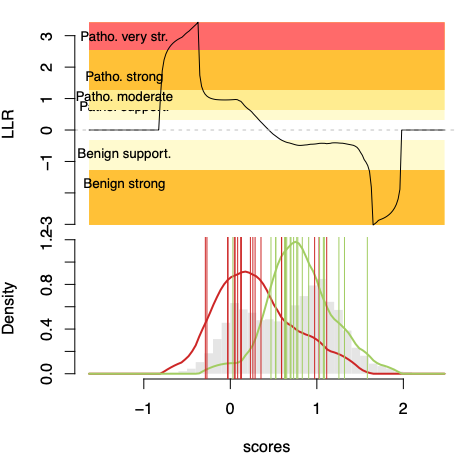
\includegraphics[width=.45\textwidth]{Figures/MTHFR/f12AV_LLR.png} }}%
    \qquad
    \subfloat[\centering f25AV]{{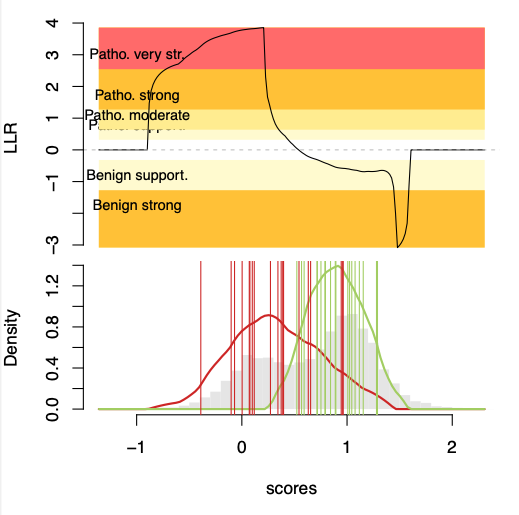
\includegraphics[width=.45\textwidth]{Figures/MTHFR/f25AV_LLR.png} }}%
    \qquad
    \subfloat[\centering f100AV]{{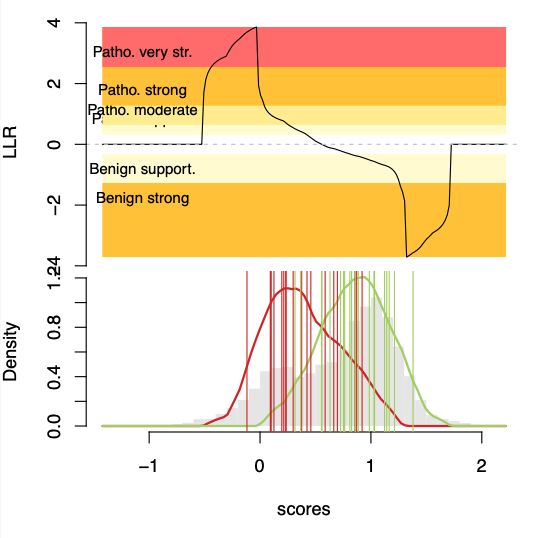
\includegraphics[width=.45\textwidth]{Figures/MTHFR/f100AV_LLR.png} }}%
    \qquad
    \subfloat[\centering f200AV]{{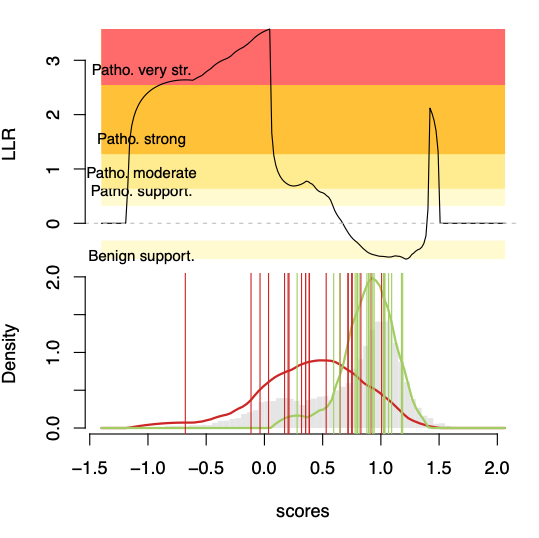
\includegraphics[width=.45\textwidth]{Figures/MTHFR/f200AV_LLR.png} }}%
    \caption{LLR of pathogenicity of MTHFR variants in A222V background, separated by different folate concentrations.}%
    \label{fig:LLR MTHFR}%
\end{figure}




% \bibliographystyle{unsrt}
% \bibliography{reference}



\end{document}